\section{Астатизм первого порядка. I регулятор}

Рассмотрим замкнутую системы с объектом управления, описываемым передаточной функцией:
\begin{equation}
    W(s) = \frac{3}{s^2 + 7.5s + 2}
\end{equation}

И регулятором, описываемым передаточной функцией:
\begin{equation}
    H(s) = \frac{k}{s}
\end{equation}
Найдем передаточную функцию замкнутой системы:
\begin{equation}
    W_{u\rightarrow y}(s) = \frac{W(s)H(s)}{1 + W(s)H(s)} = \frac{3k}{s(s^2 + 7.5s + 2) + 3k}
\end{equation}
Согласно следствию из критерия Гурвица для систем третьего порядка, система будет устойчива при:
\begin{equation}
    \begin{cases}
        7.5 > 0 \\
        2 > 0 \\ 
        3k > 0 \\ 
        7.5 \cdot 2 > 3k \\
    \end{cases} \Rightarrow
    k < 5
\end{equation}

Найдем передаточную функцию по ошибке:
\begin{equation}
    W_{u\rightarrow e}(s) = \frac{1}{1 + W(s)H(s)} = \frac{s(s^2 + 7.5s + 2)}{s(s^2 + 7.5s + 2) + 3k}
\end{equation}

\subsection{Статическая система}
Найдем образ Лапласа входного воздействия:
\begin{equation}
    L\{A\} = \frac{A}{s}
\end{equation}
Теперь найдем образ Лапласа ошибки:
\begin{equation}
    E = W_{u\rightarrow e}(s)L\{A\} = \frac{s(s^2 + 7.5s + 2)}{s(s^2 + 7.5s + 2) + 3k}\frac{A}{s} = \frac{A(s^2 + 7.5s + 2)}{s^2 + 7.5s + 2 + 3k}
\end{equation}
Согласно теореме о конечном значении, установившееся значение ошибки равно:
\begin{equation}
    e_{\text{set}} = \lim_{s \to 0} sE = \lim_{s \to 0} \frac{A(s^2 + 7.5s + 2)}{s^2 + 7.5s + 2 + 3k} = \frac{2sA}{3k} = 0 
\end{equation}

% Возьмем $k = 0.1$. Таким образом, согласно теоретическим расчетам, система будет устойчива. Промоделируем (см рис. \ref{fig:task4_out}).
% График ошибки приведен на рис. \ref{fig:task4_error}. Теоретическое значение установившегося значения ошибки: $e_{\text{set}} = 0$.
% Фактическое значение установившегося значения ошибки: $e_{\text{set}} = 0.0$.

% \begin{figure}[ht!]
%     \centering
%     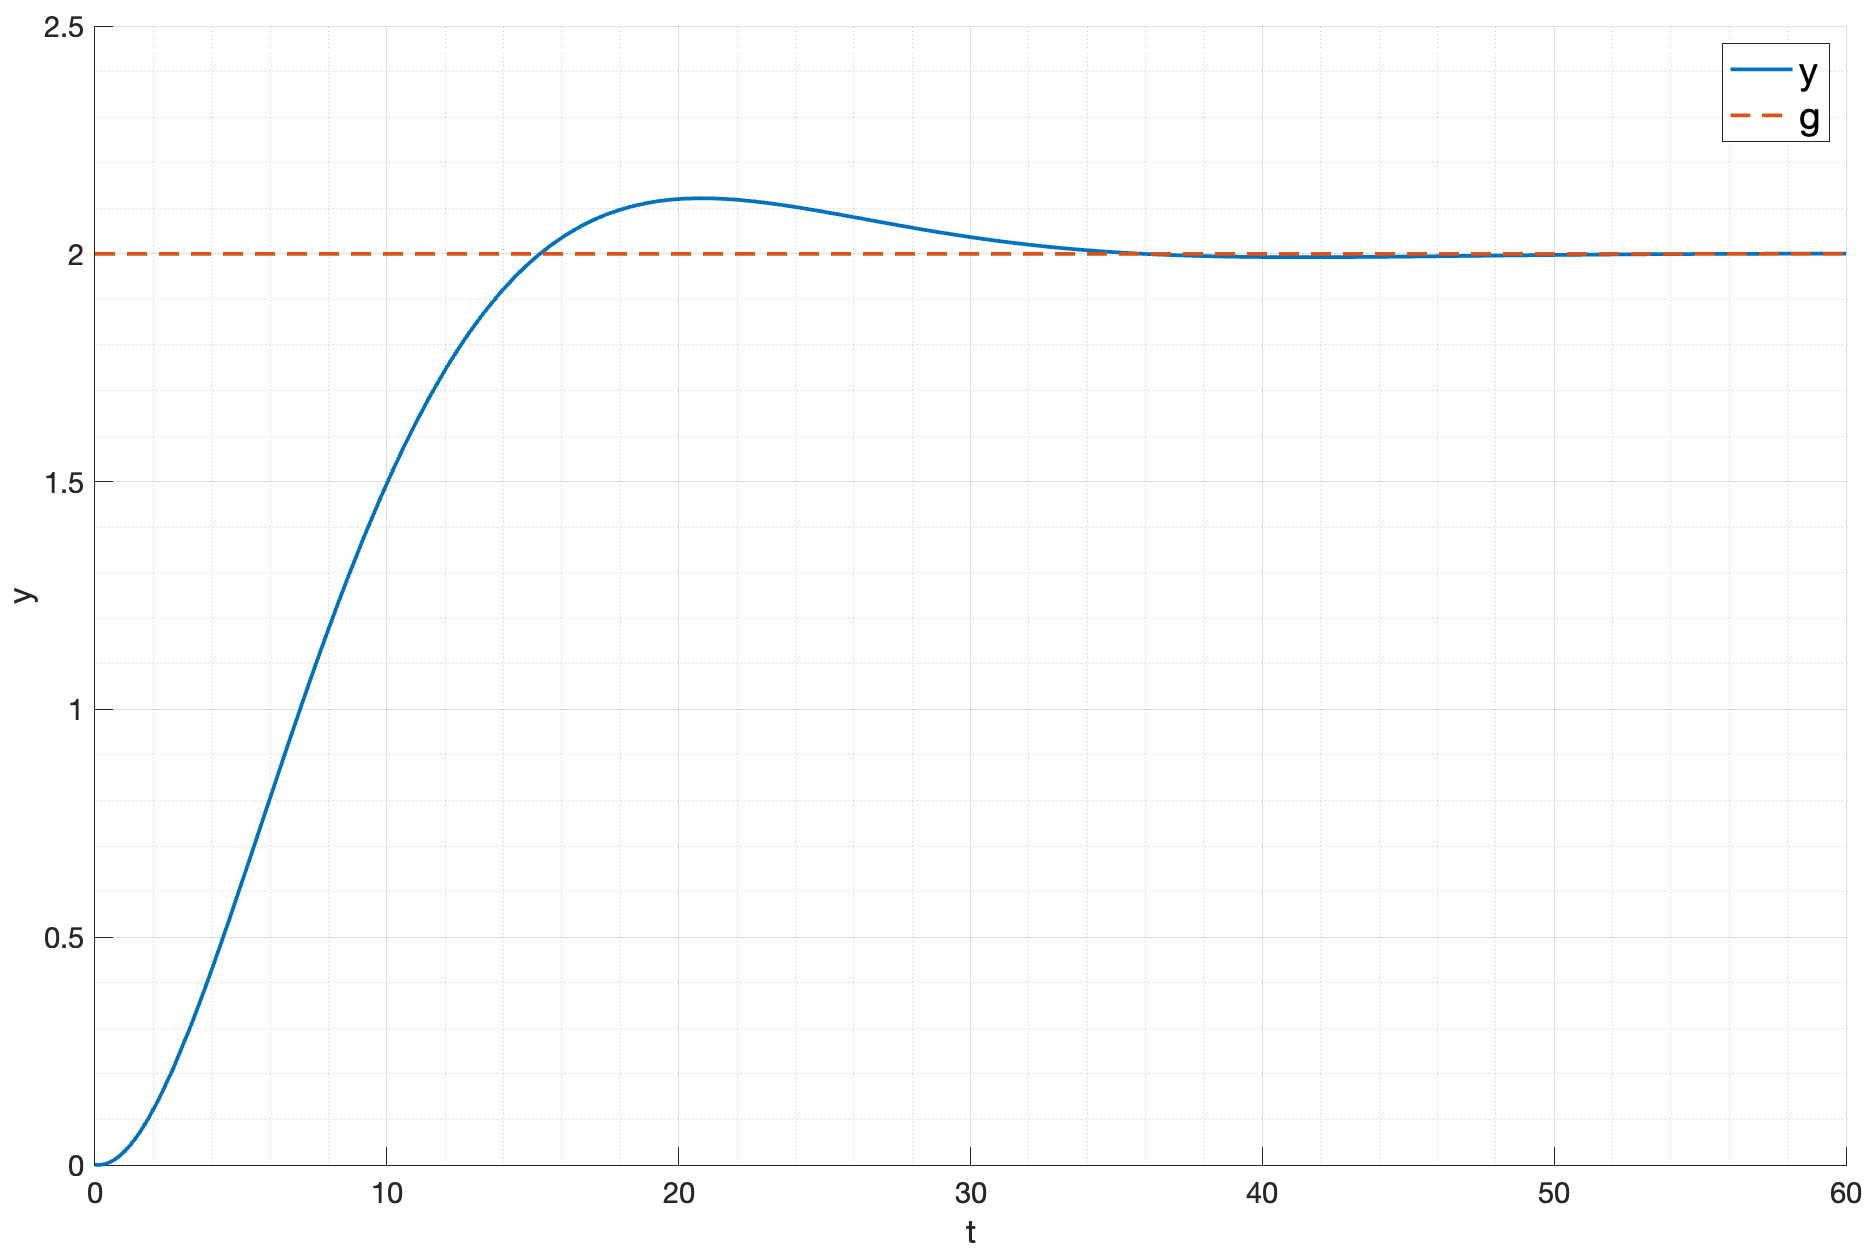
\includegraphics[width=\textwidth]{"media/plots/task4_out.png"}
%     \caption{Моделирование системы с I регулятором ($k = 0.1$) ($u(t) = A$)}
%     \label{fig:task4_out}
% \end{figure}

% \begin{figure}
%     \centering
%     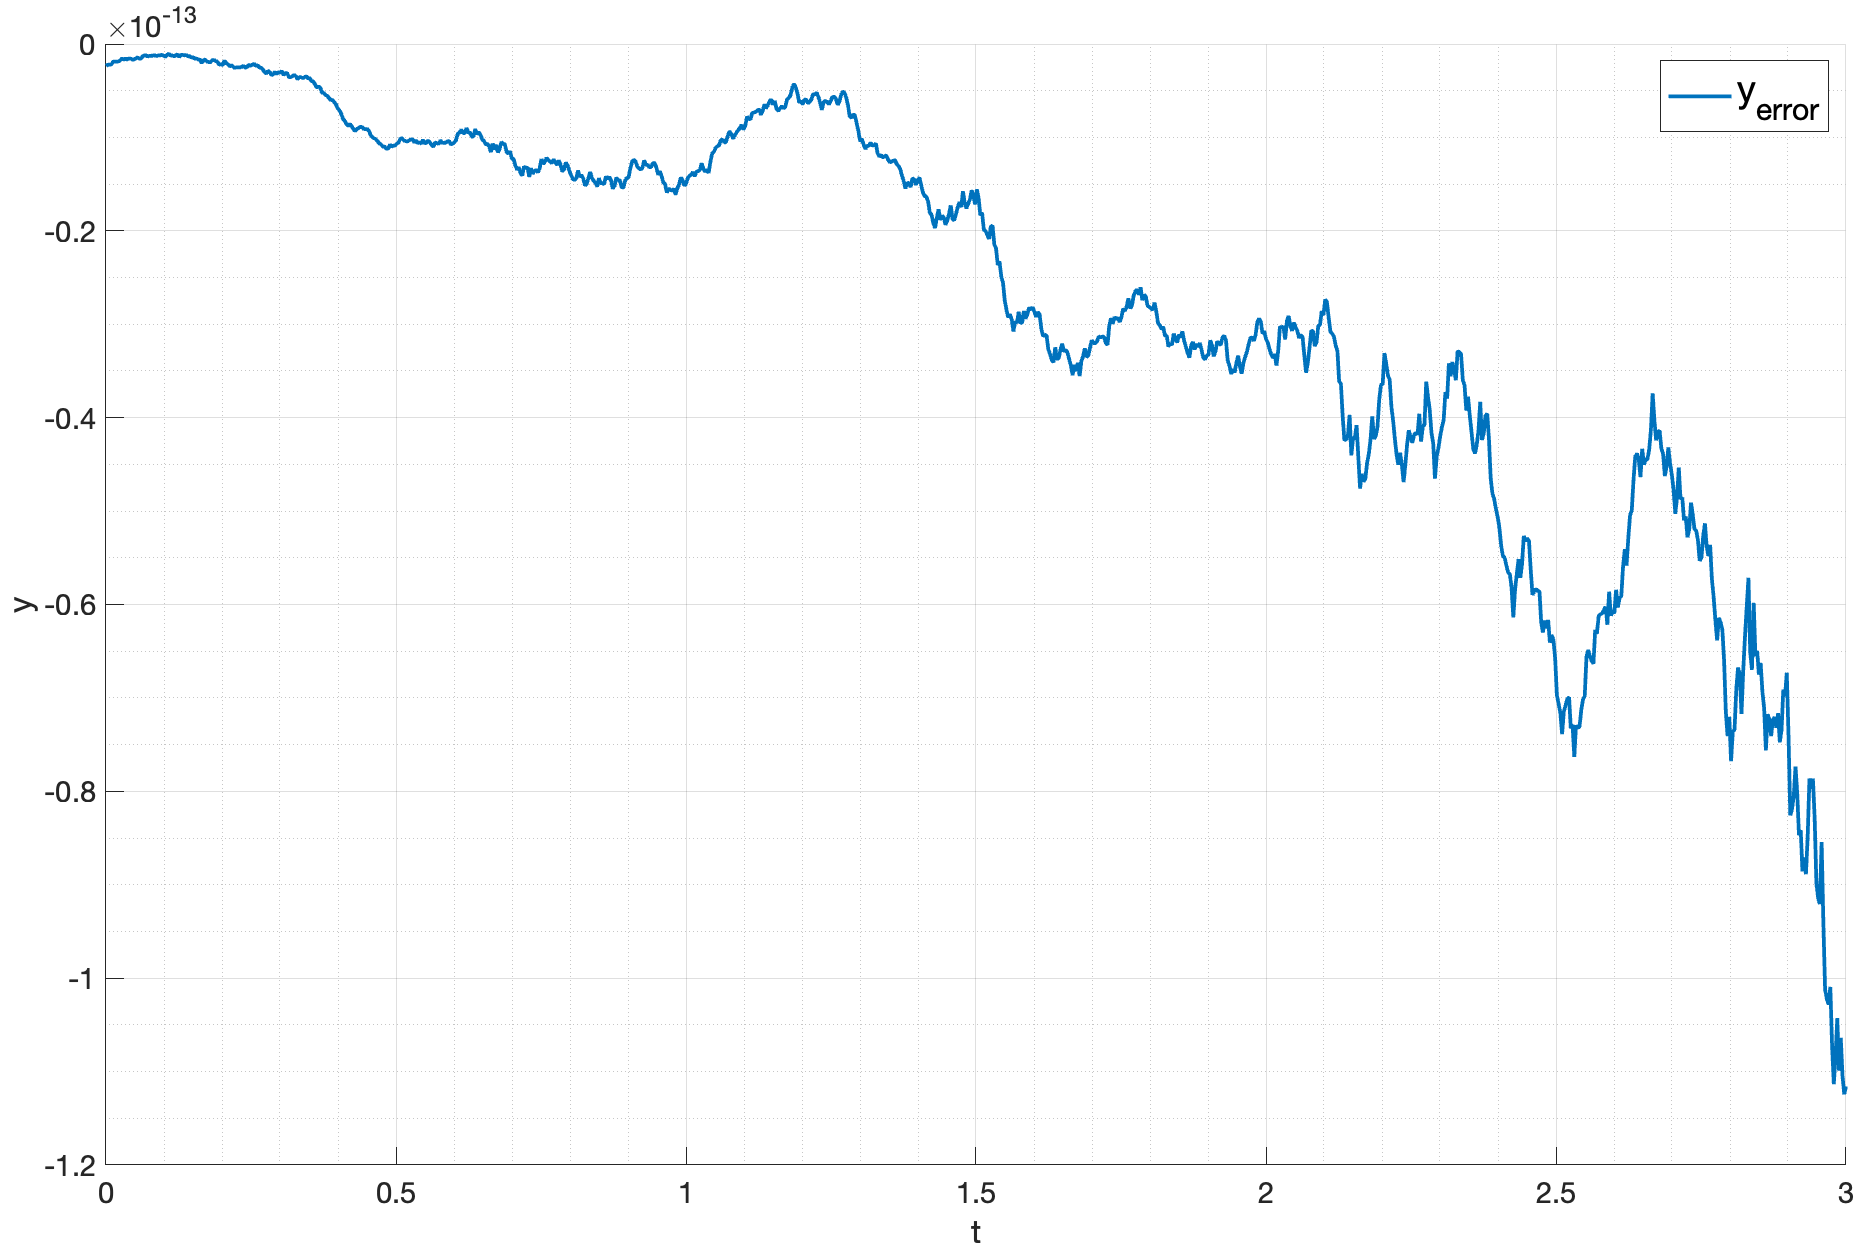
\includegraphics[width=\textwidth]{"media/plots/task4_error.png"}
%     \caption{График ошибки системы с I регулятором ($k = 0.1$) ($u(t) = A$)}
%     \label{fig:task4_error}
% \end{figure}

% Возьмем $k = 0.3$. Таким образом, согласно теоретическим расчетам, система будет устойчива. Промоделируем (см рис. \ref{fig:task4_out2}).
% График ошибки приведен на рис. \ref{fig:task4_error2}. Теоретическое значение установившегося значения ошибки: $e_{\text{set}} = 0$.
% Фактическое значение установившегося значения ошибки: $e_{\text{set}} = 0.0$.

% \begin{figure}[ht!]
%     \centering
%     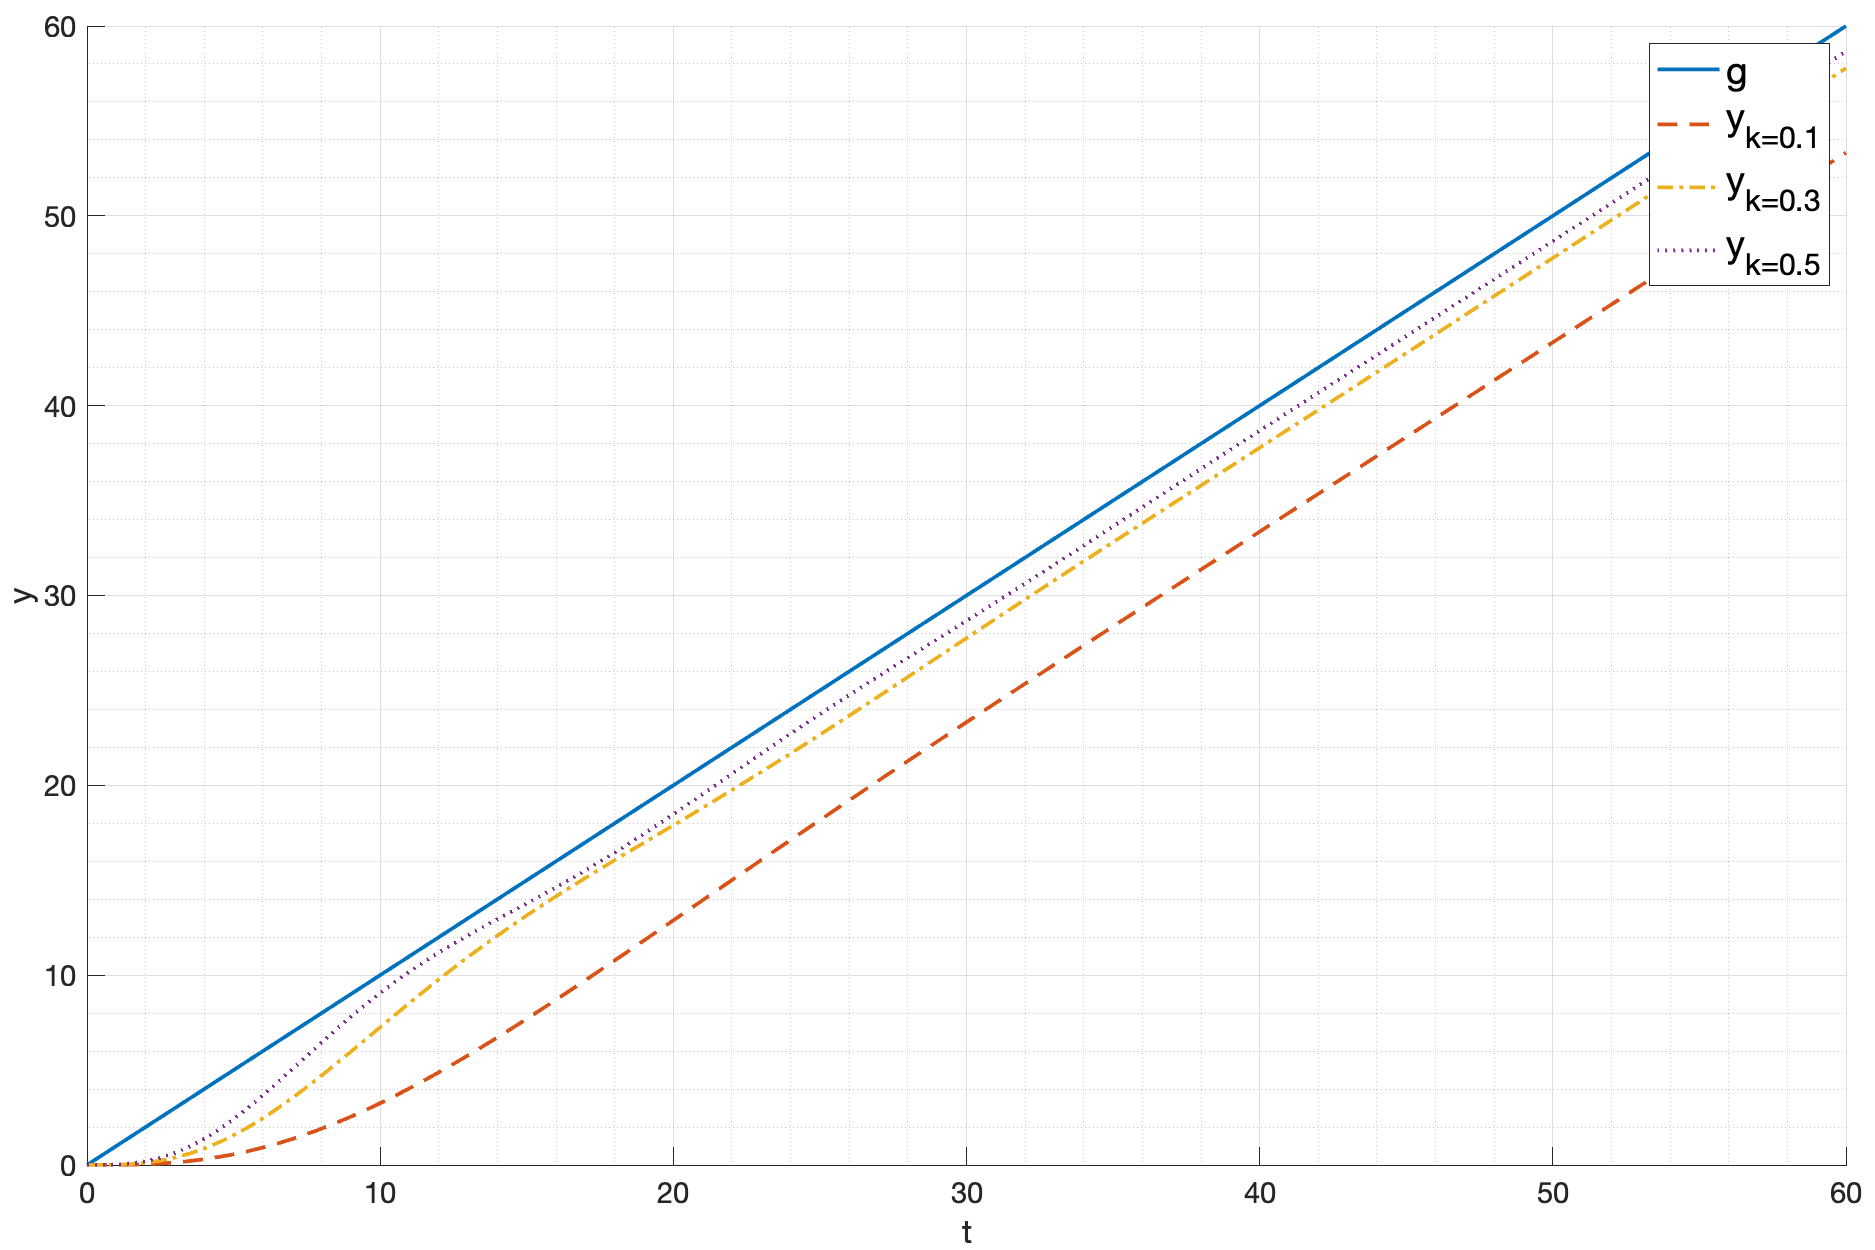
\includegraphics[width=\textwidth]{"media/plots/task4_out2.png"}
%     \caption{Моделирование системы с I регулятором ($k = 0.3$) ($u(t) = A$)}
%     \label{fig:task4_out2}
% \end{figure}

% \begin{figure}
%     \centering
%     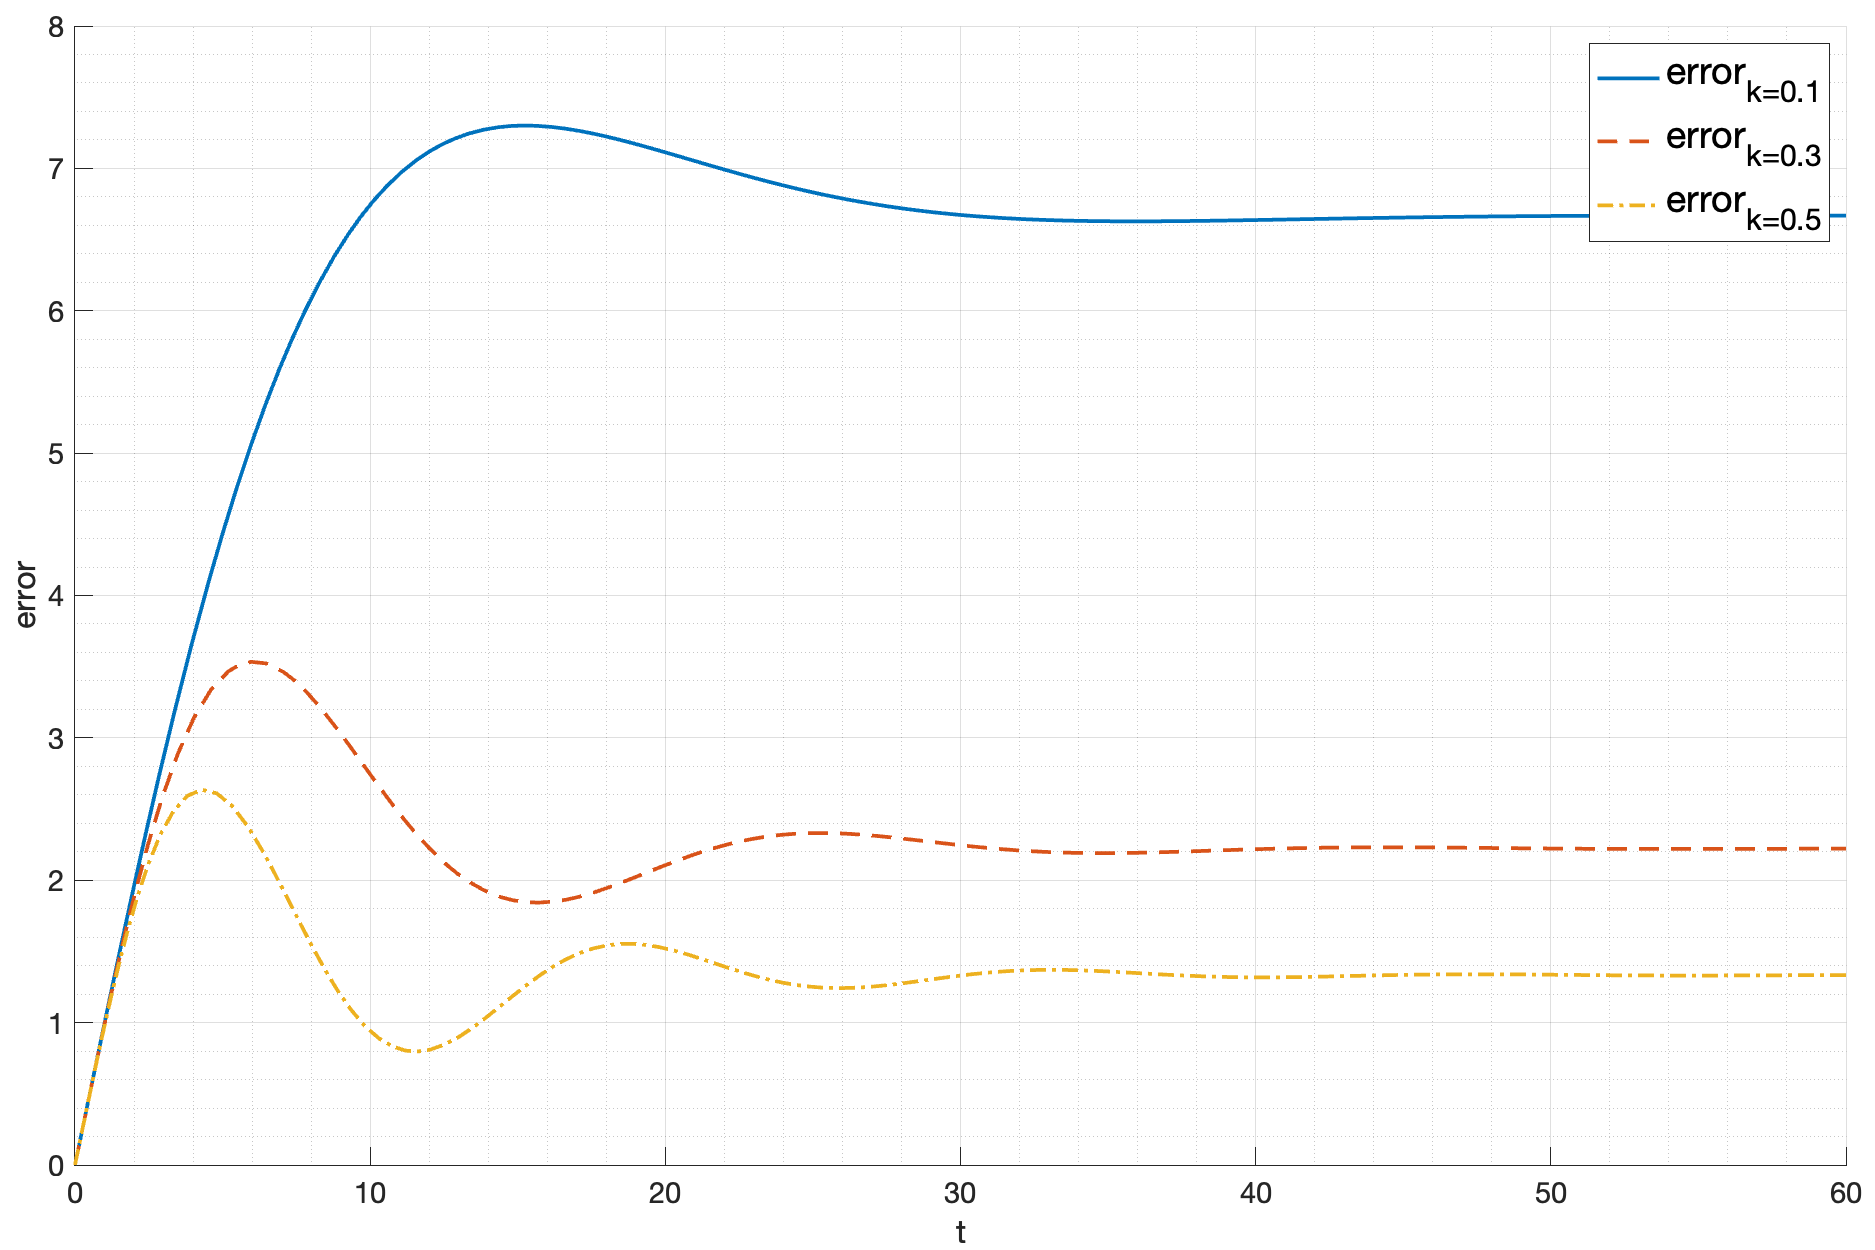
\includegraphics[width=\textwidth]{"media/plots/task4_error2.png"}
%     \caption{График ошибки системы с I регулятором ($k = 0.3$) ($u(t) = A$)}
%     \label{fig:task4_error2}
% \end{figure}

% Возьмем $k = 0.5$. Таким образом, согласно теоретическим расчетам, система будет устойчива. Промоделируем (см рис. \ref{fig:task4_out3}).
% График ошибки приведен на рис. \ref{fig:task4_error3}. Теоретическое значение установившегося значения ошибки: $e_{\text{set}} = 0$.
% Фактическое значение установившегося значения ошибки: $e_{\text{set}} = 0.0$.

% \begin{figure}[ht!]
%     \centering
%     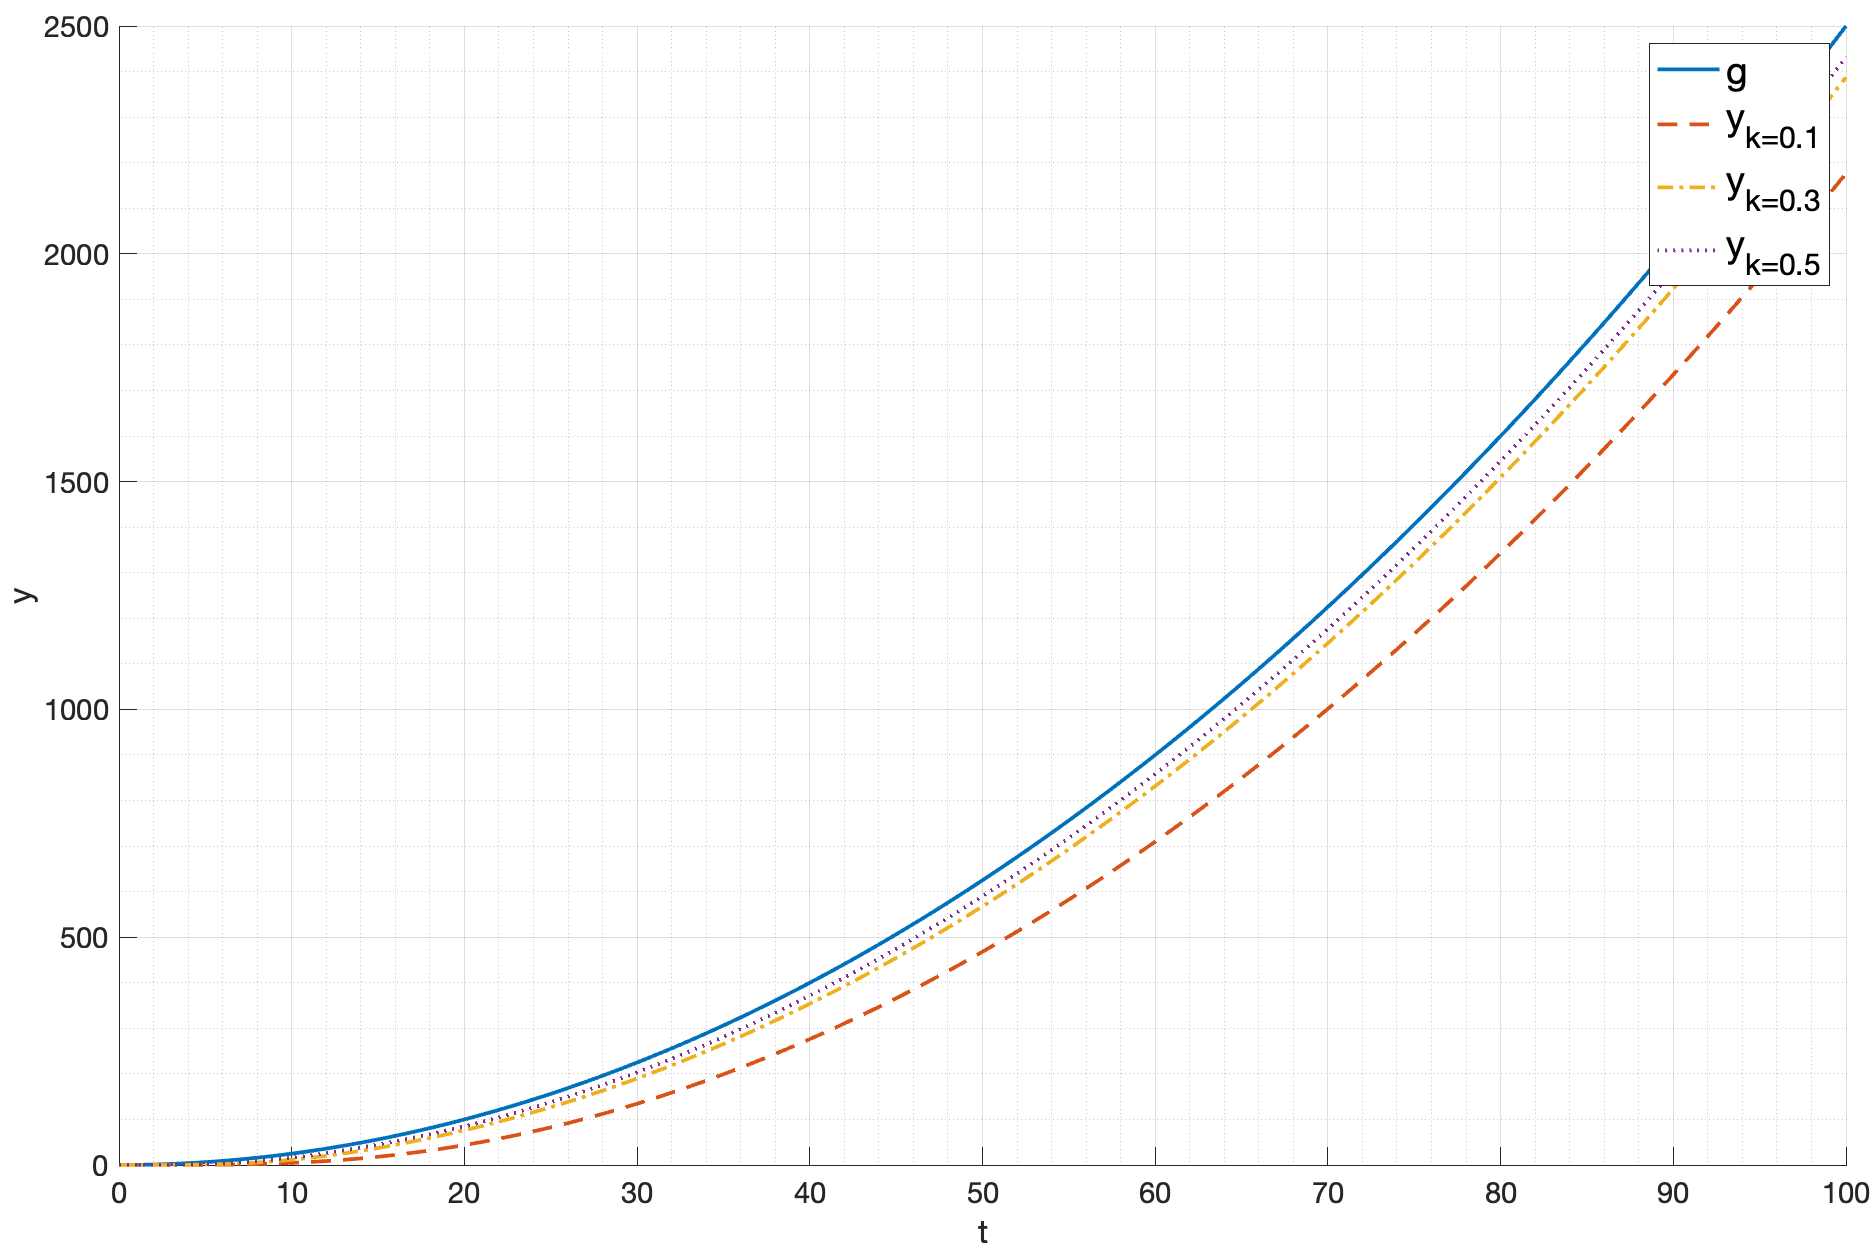
\includegraphics[width=\textwidth]{"media/plots/task4_out3.png"}
%     \caption{Моделирование системы с I регулятором ($k = 0.5$) ($u(t) = A$)}
%     \label{fig:task4_out3}
% \end{figure}

% \begin{figure}
%     \centering
%     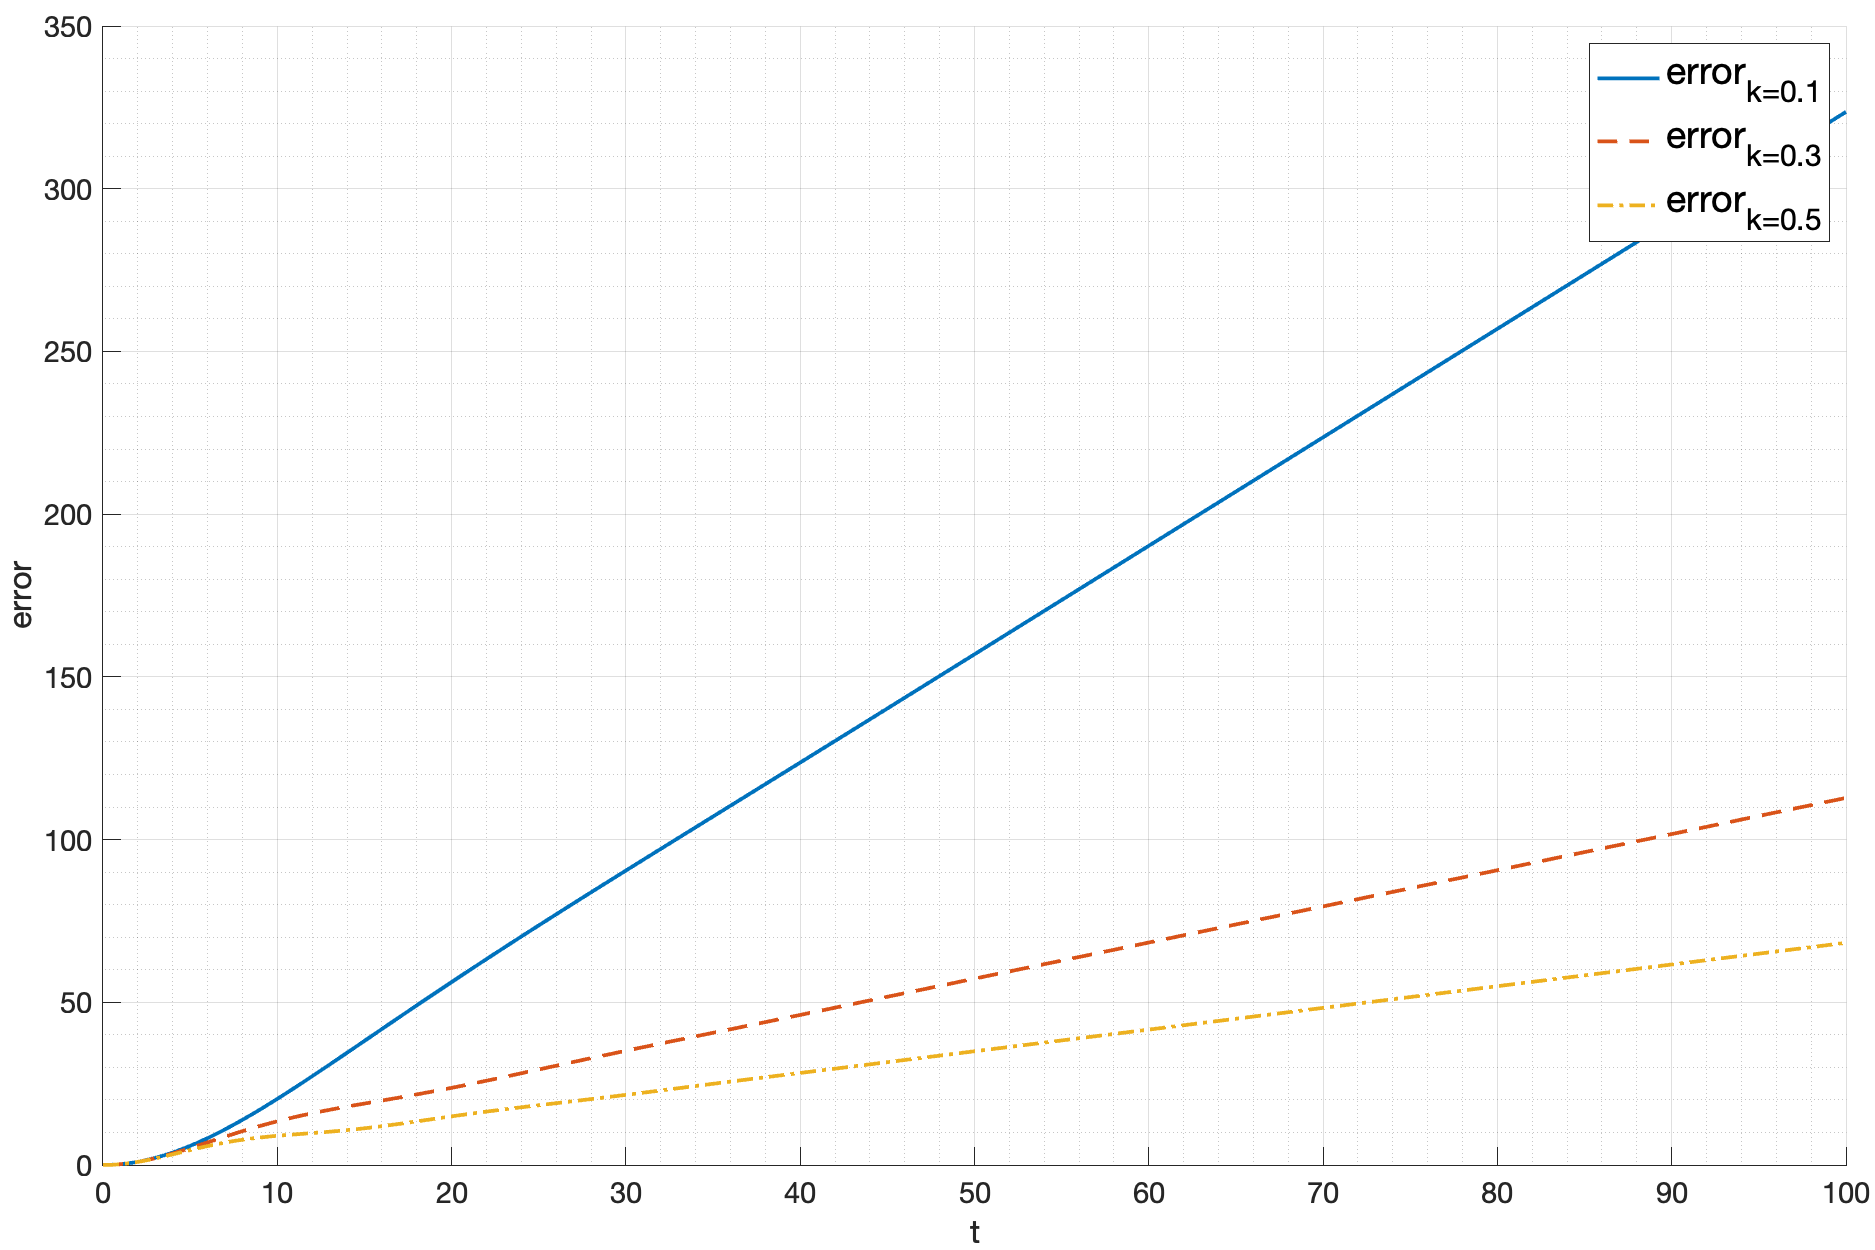
\includegraphics[width=\textwidth]{"media/plots/task4_error3.png"}
%     \caption{График ошибки системы с I регулятором ($k = 0.5$) ($u(t) = A$)}
%     \label{fig:task4_error3}
% \end{figure}

Проведем моделирование системы с линейно возрастающим входным воздействием при значениях $k = \{0.1, 0.3, 0.5\}$.
Результаты моделирования приведены на рис. \ref{fig:task4_out}, \ref{fig:task4_error}.

\begin{table}
    \centering
    \begin{tabular}{|c|c|c|}
        \hline
        $k$ & $e_{\text{set}}$ & $e_{\text{fact}}$ \\
        \hline
        0.1 & 0 & 0.0 \\
        0.3 & 0 & 0.0 \\
        0.5 & 0 & 0.0 \\
        \hline
    \end{tabular}
    \caption{Сравнение теоретического и фактического установившегося значения ошибки}
\end{table}

\begin{figure}[ht!]
    \centering
    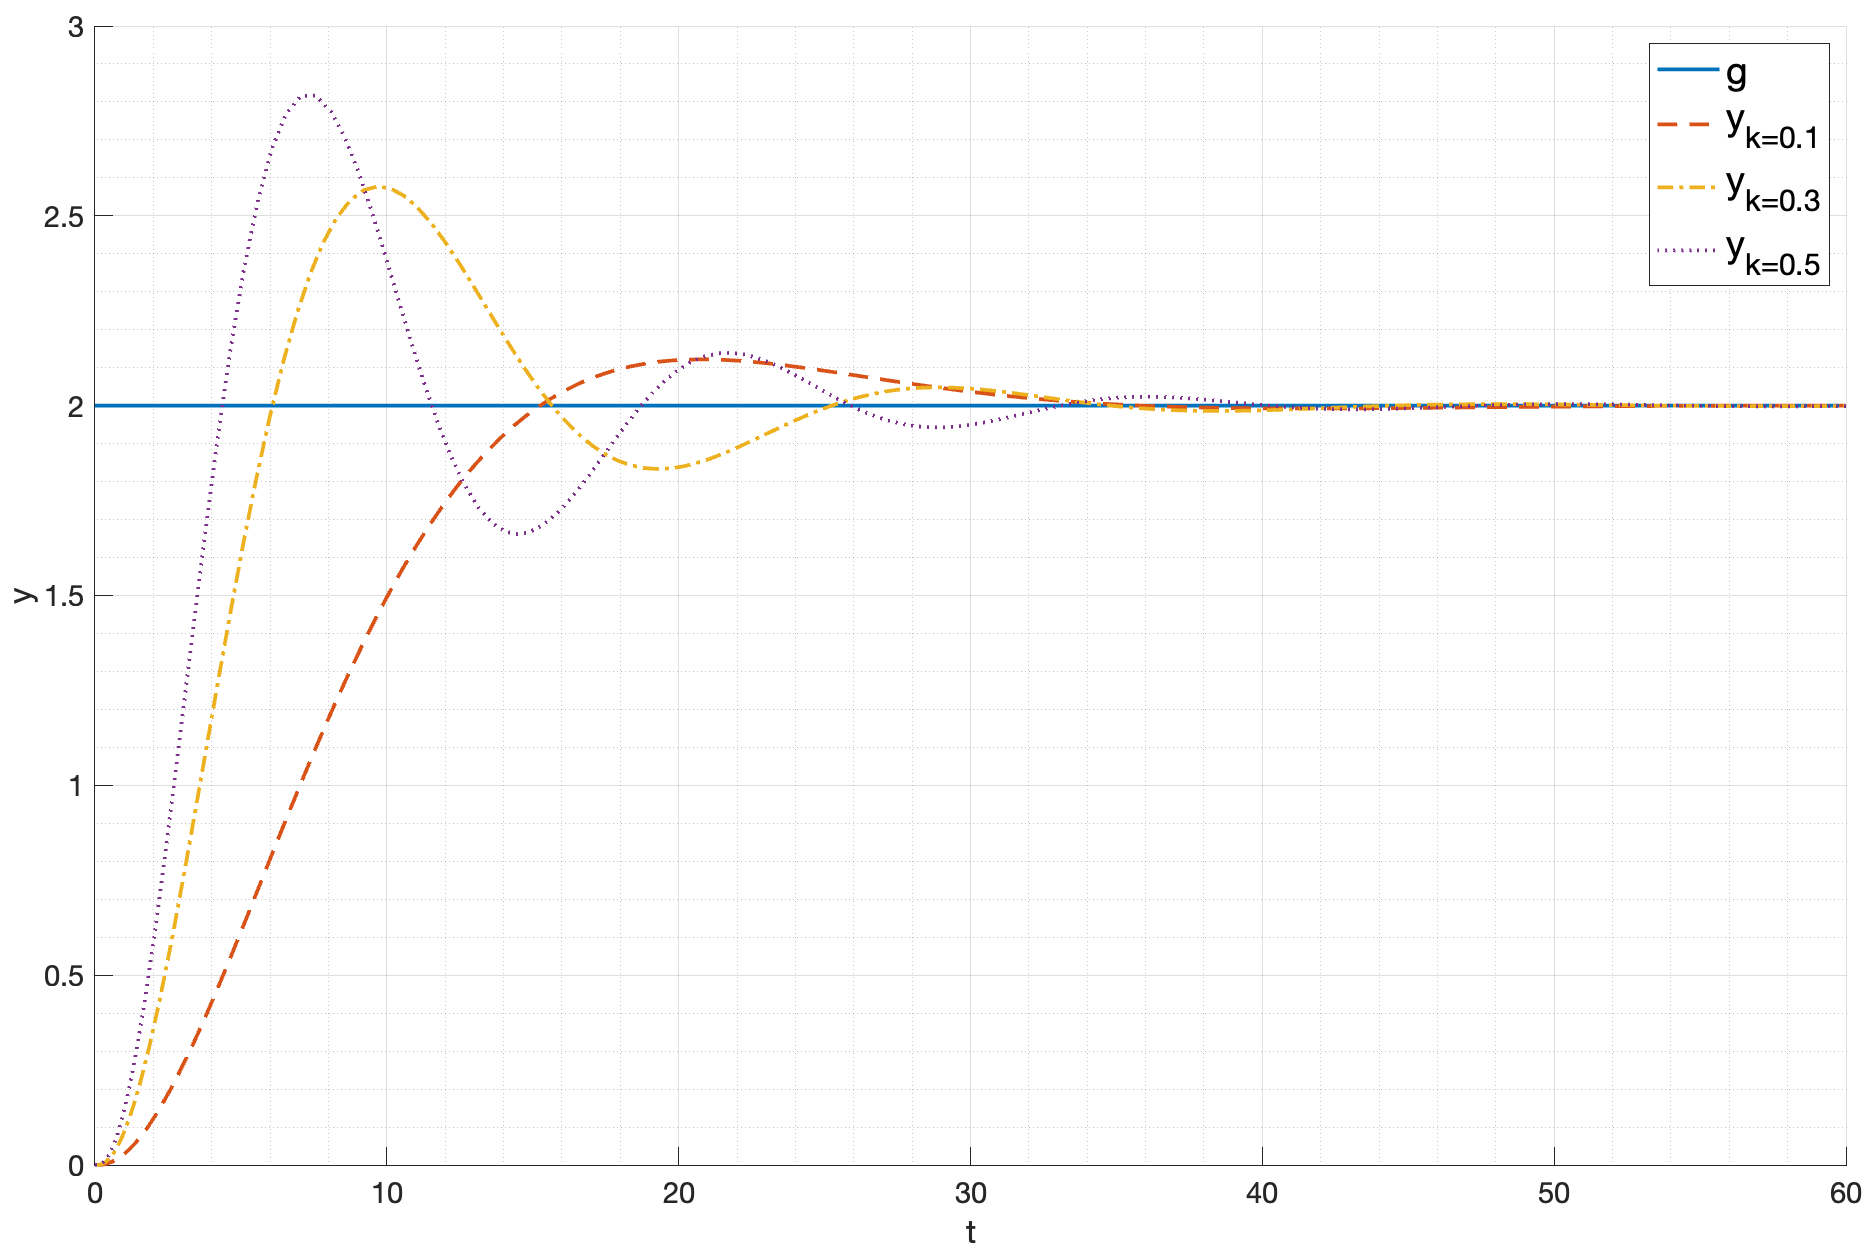
\includegraphics[width=\textwidth]{"media/plots/task4_out1.png"}
    \caption{Моделирование системы с I регулятором ($u(t) = Vt$)}
    \label{fig:task4_out}
\end{figure}

\begin{figure}[ht!]
    \centering
    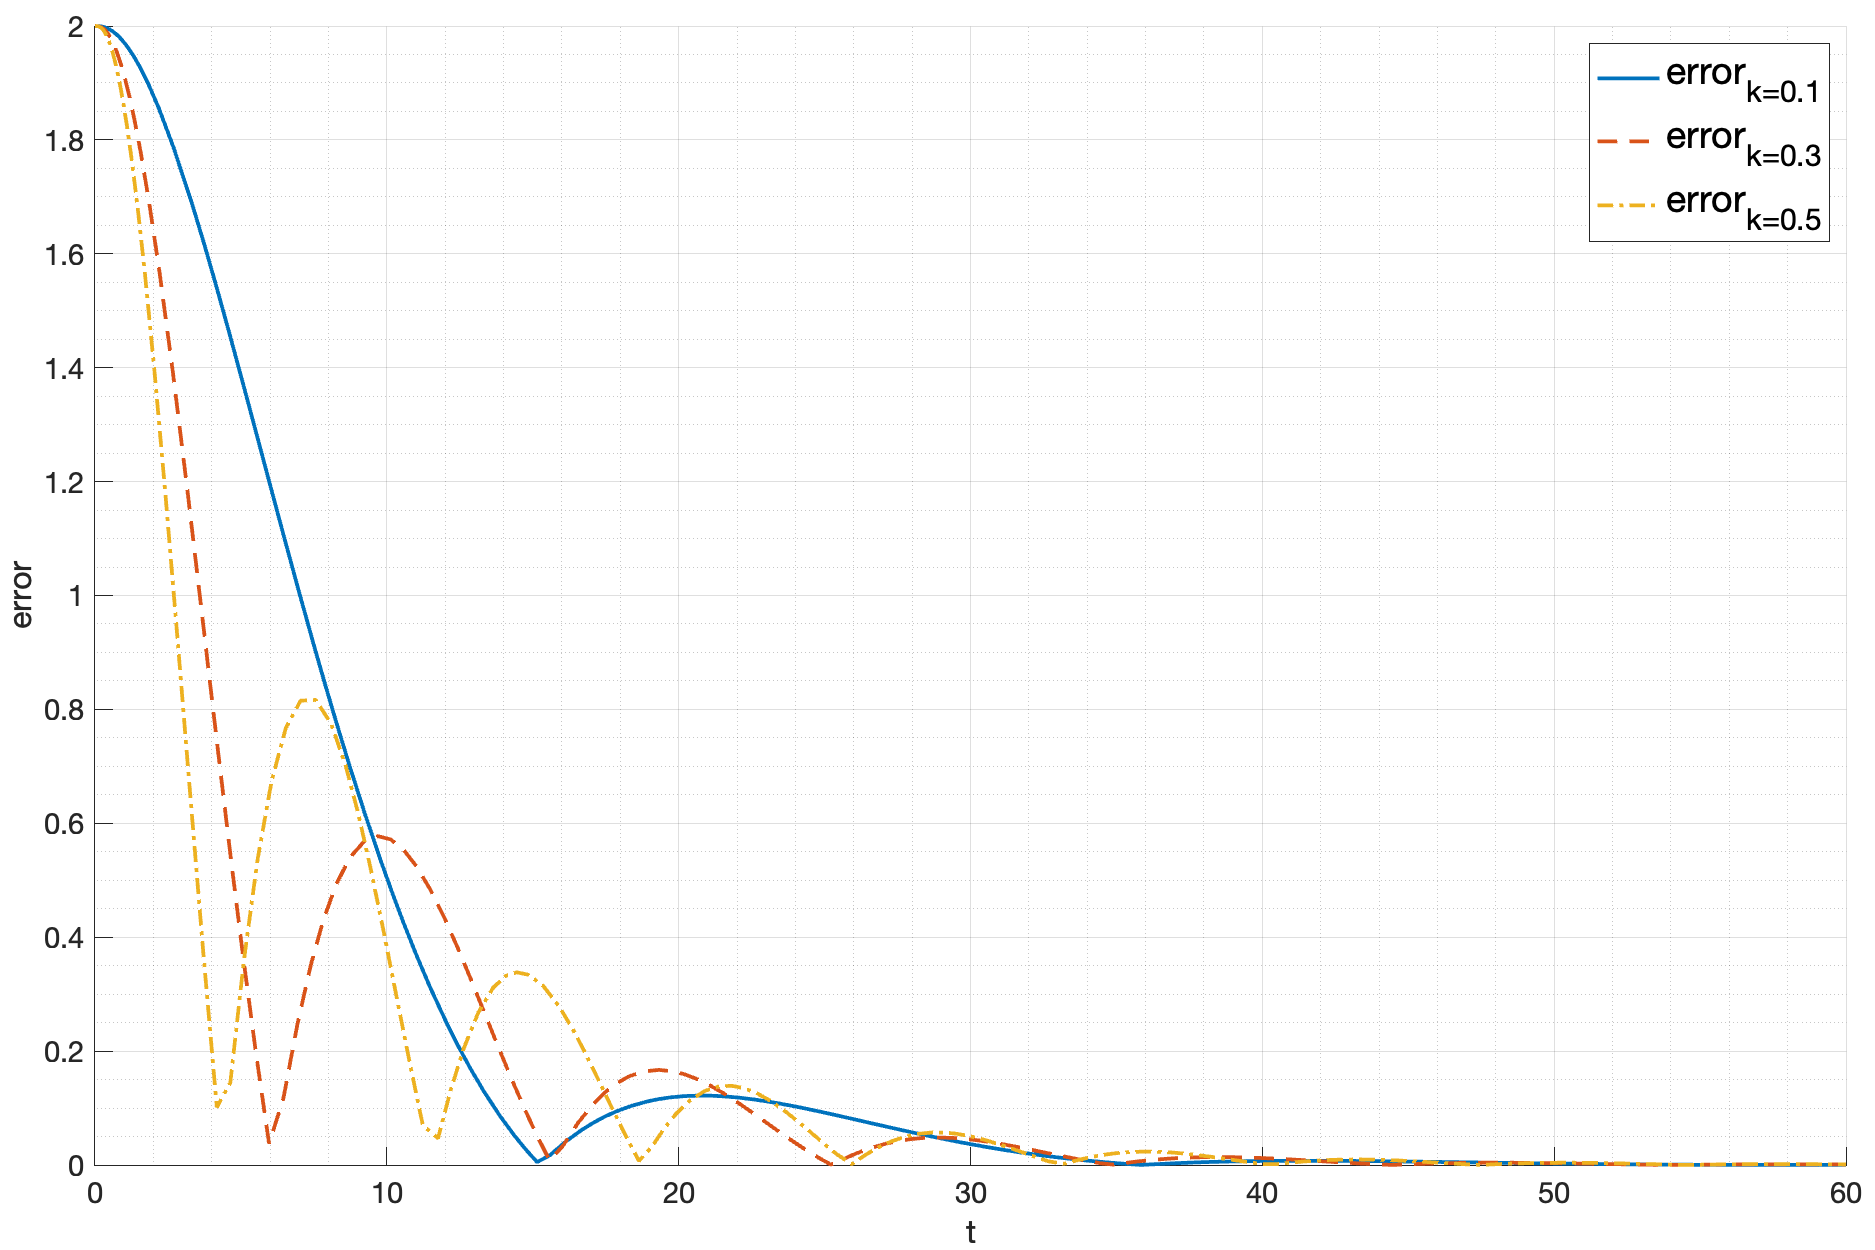
\includegraphics[width=\textwidth]{"media/plots/task4_error1.png"}
    \caption{График ошибки системы с I регулятором ($u(t) = Vt$)}
    \label{fig:task4_error}
\end{figure}


Видно, что во всех трех случаях система устойчива и ошибки стремятся к нулю, что соответствует теоретическим расчетам.

\subsection{Система с линейно возрастающим входным воздействием}
Рассмотрим систему с линейно возрастающим входным воздействием:
\begin{equation}
    u(t) = Vt
\end{equation}
Найдем образ Лапласа входного воздействия:
\begin{equation}
    L\{u\} = \frac{V}{s^2}
\end{equation}
Найдем образ Лапласа ошибки:
\begin{equation}
    E = W_{u\rightarrow e}(s)L\{u\} = \frac{s(s^2 + 7.5s + 2)}{s(s^2 + 7.5s + 2) + 3k}\frac{V}{s^2} = \frac{V(s^2 + 7.5s + 2)}{s(s(s^2 + 7.5s + 2) + 3k)}
\end{equation}
Согласно теореме о конечном значении, установившееся значение ошибки равно:
\begin{equation}
    e_{\text{set}} = \lim_{s \to 0} sE = \lim_{s \to 0} \frac{V(s^2 + 7.5s + 2)}{s(s^2 + 7.5s + 2) + 3k} = \frac{2V}{3k}
\end{equation}

Проведем моделирование системы с линейно возрастающим входным воздействием при значениях $k = \{0.1, 0.3, 0.5\}$.
Результаты моделирования приведены на рис. \ref{fig:task4_out2}, \ref{fig:task4_error2}.

\begin{table}[ht!]
    \centering
    \begin{tabular}{|c|c|c|}
        \hline
        $k$ & $e_{\text{set}}$ & $e_{\text{fact}}$ \\
        \hline
        0.1 & 6.67 & 6.67 \\
        0.3 & 2.22 & 2.22 \\
        0.5 & 1.33 & 1.33 \\
        \hline
    \end{tabular}
    \caption{Сравнение теоретического и фактического установившегося значения ошибки}
\end{table}

\begin{figure}[ht!]
    \centering
    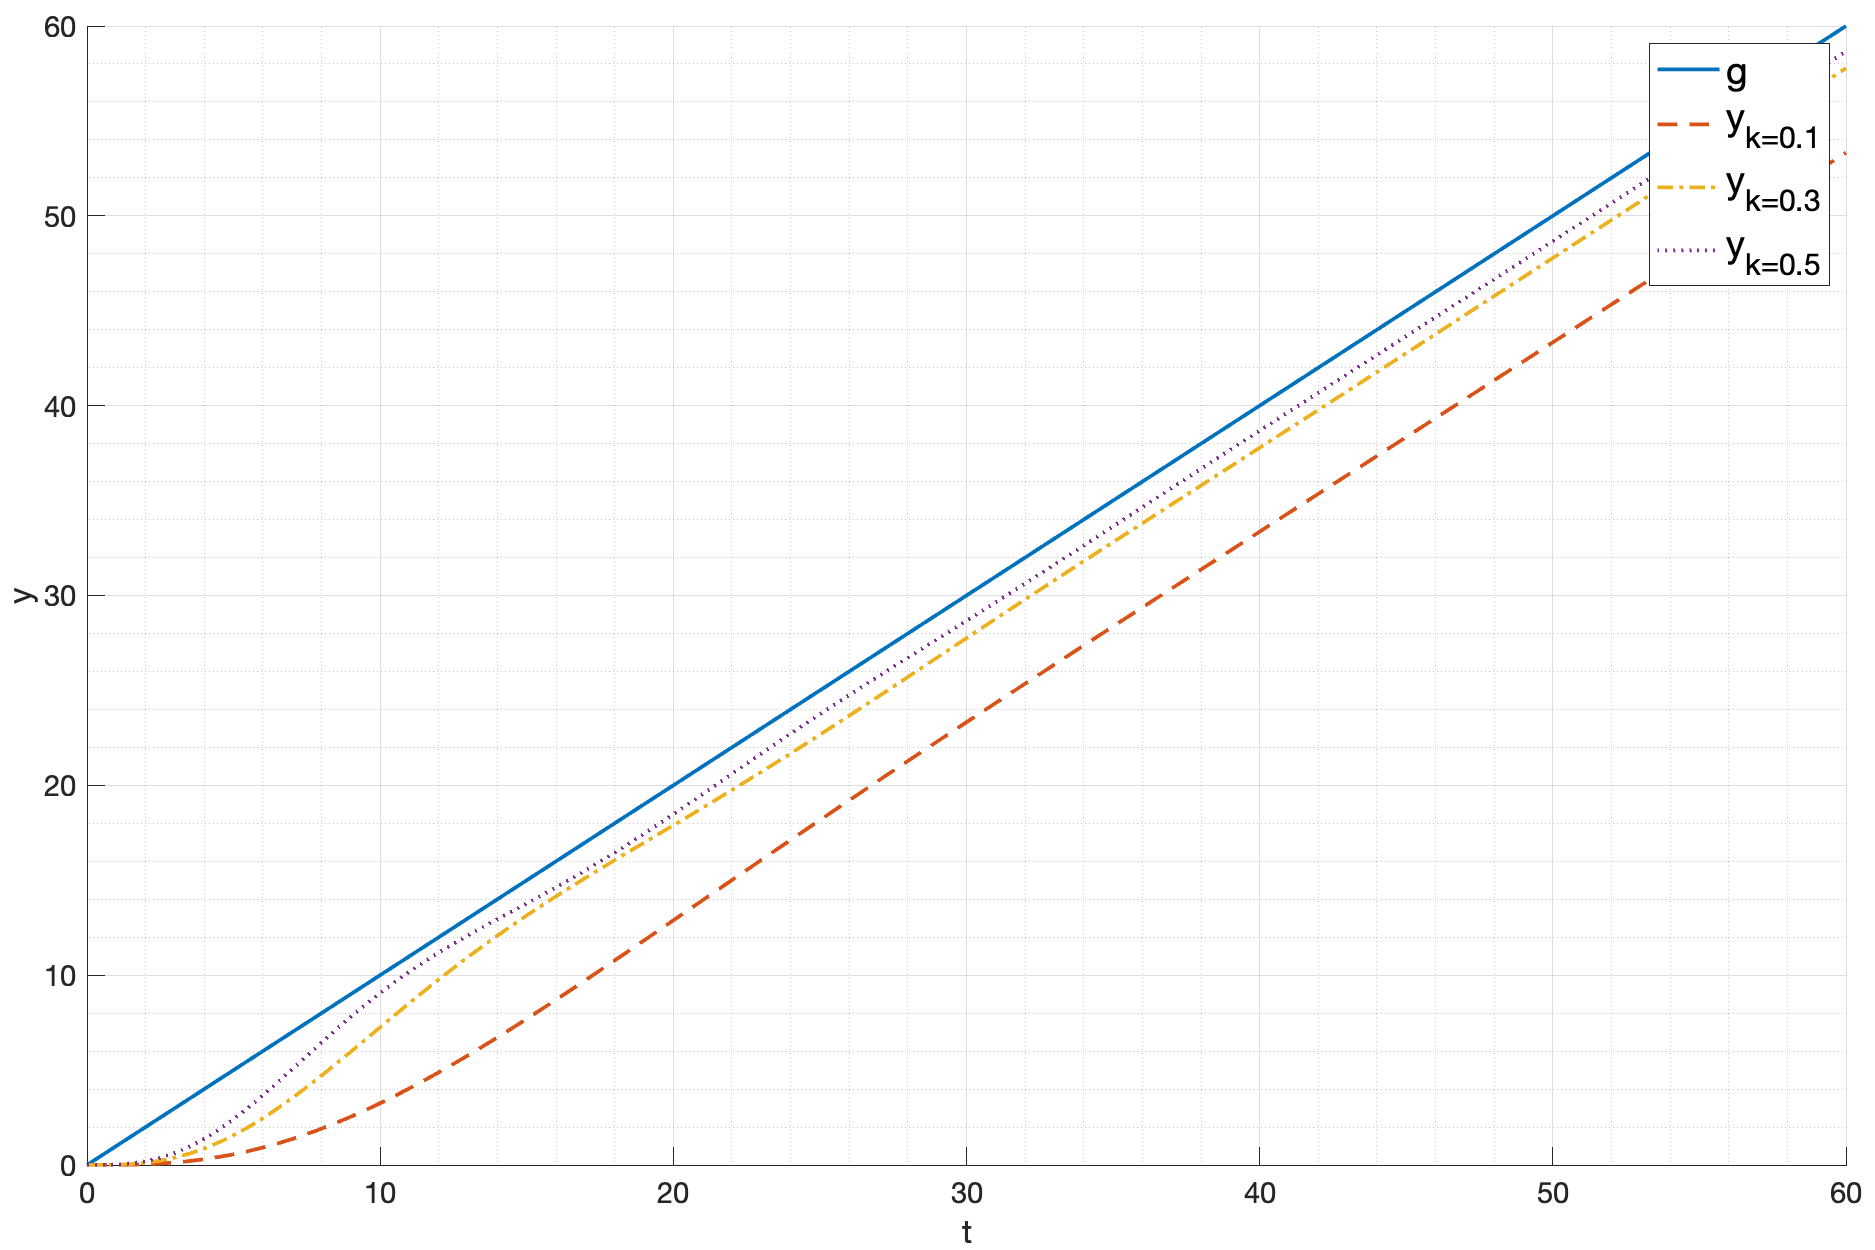
\includegraphics[width=\textwidth]{"media/plots/task4_out2.png"}
    \caption{Моделирование системы с I регулятором ($u(t) = Vt$)}
    \label{fig:task4_out2}
\end{figure}

\begin{figure}[ht!]
    \centering
    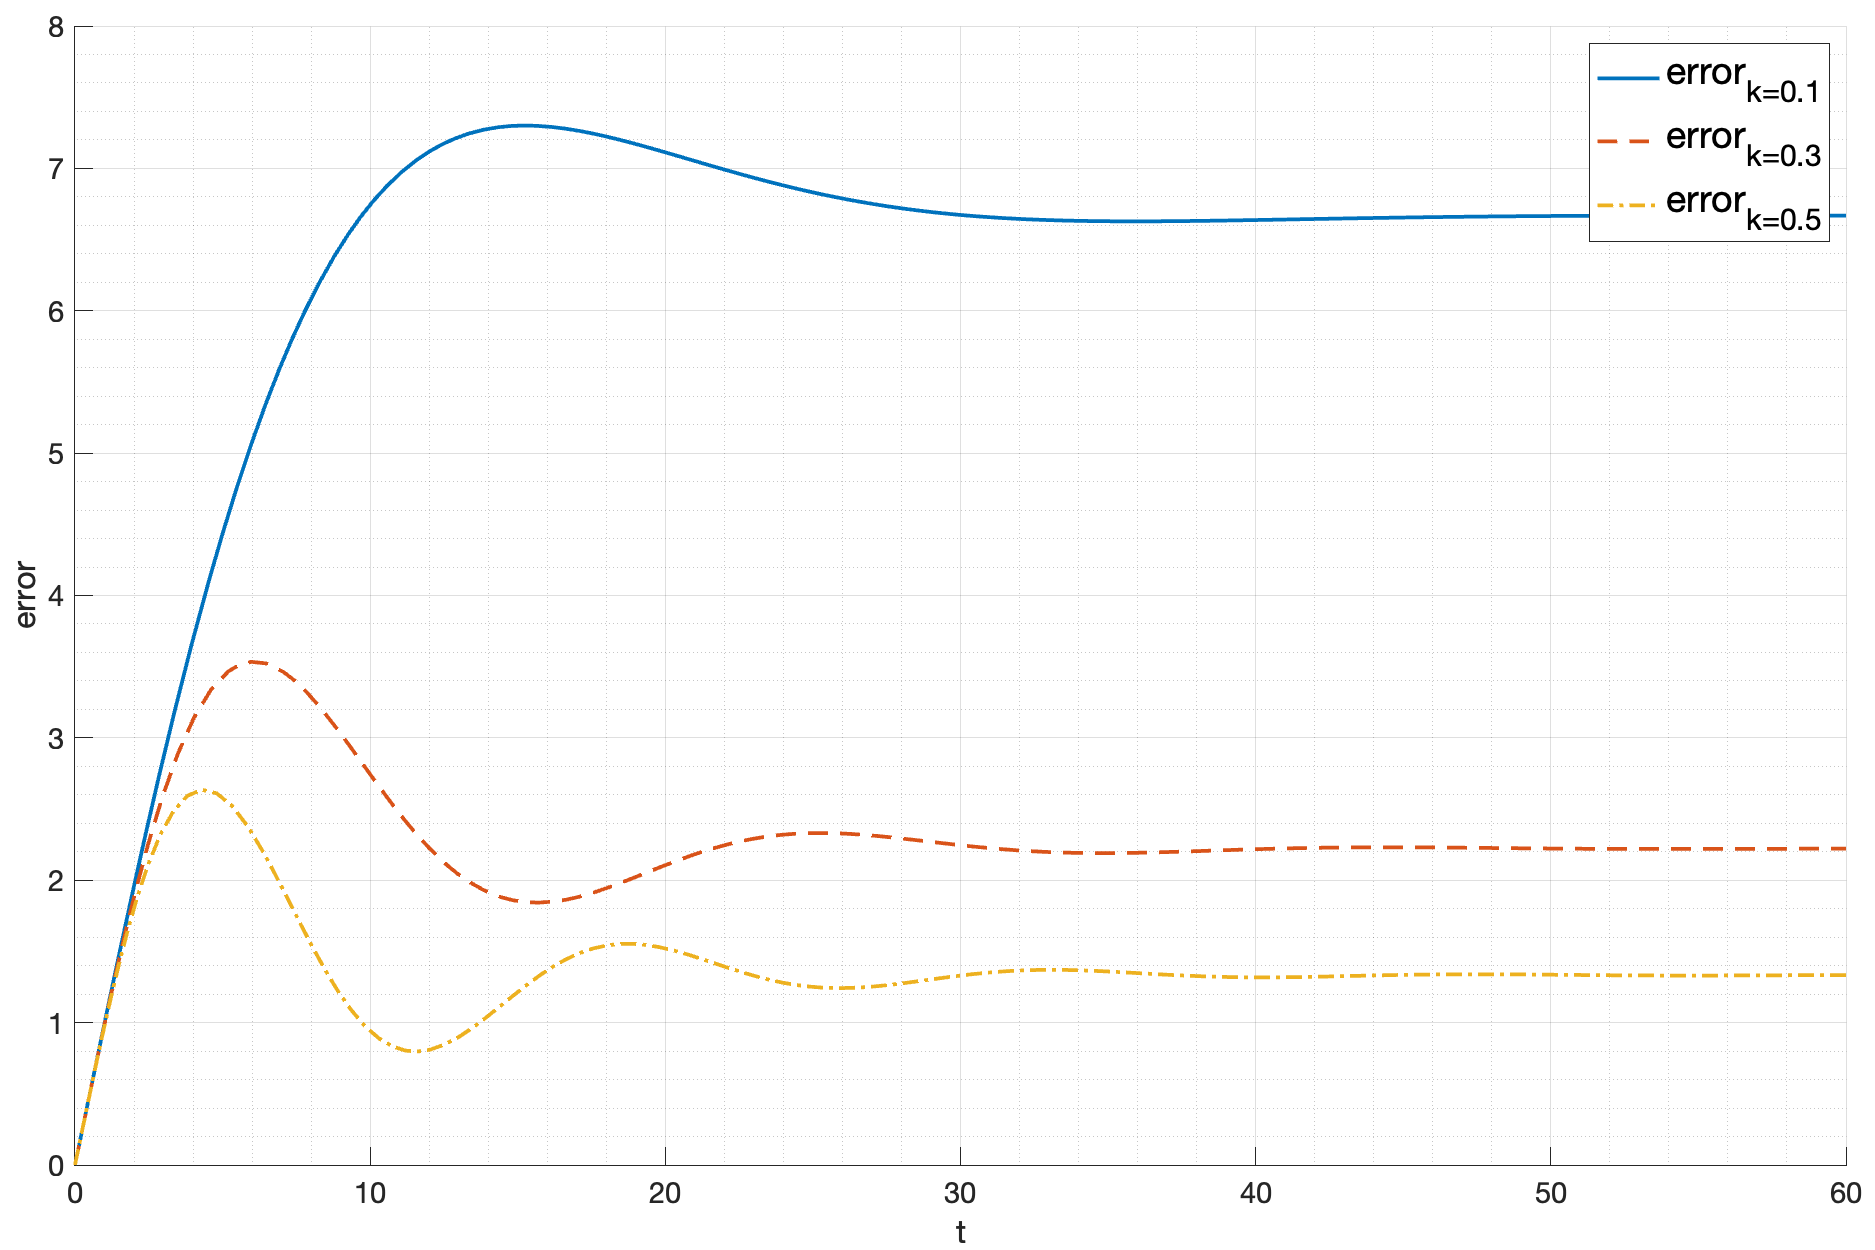
\includegraphics[width=\textwidth]{"media/plots/task4_error2.png"}
    \caption{График ошибки системы с I регулятором ($u(t) = Vt$)}
    \label{fig:task4_error2}
\end{figure}

% Возьмем $k = 0.1$. Таким образом, согласно теоретическим расчетам, система будет устойчива. Промоделируем (см рис. \ref{fig:task4_out4}).
% График ошибки приведен на рис. \ref{fig:task4_error4}. Теоретическое значение установившегося значения ошибки: $e_{\text{set}} = 6.6$.
% Фактическое значение установившегося значения ошибки: $e_{\text{set}} = 6.67$.

% \begin{figure}[ht!]
%     \centering
%     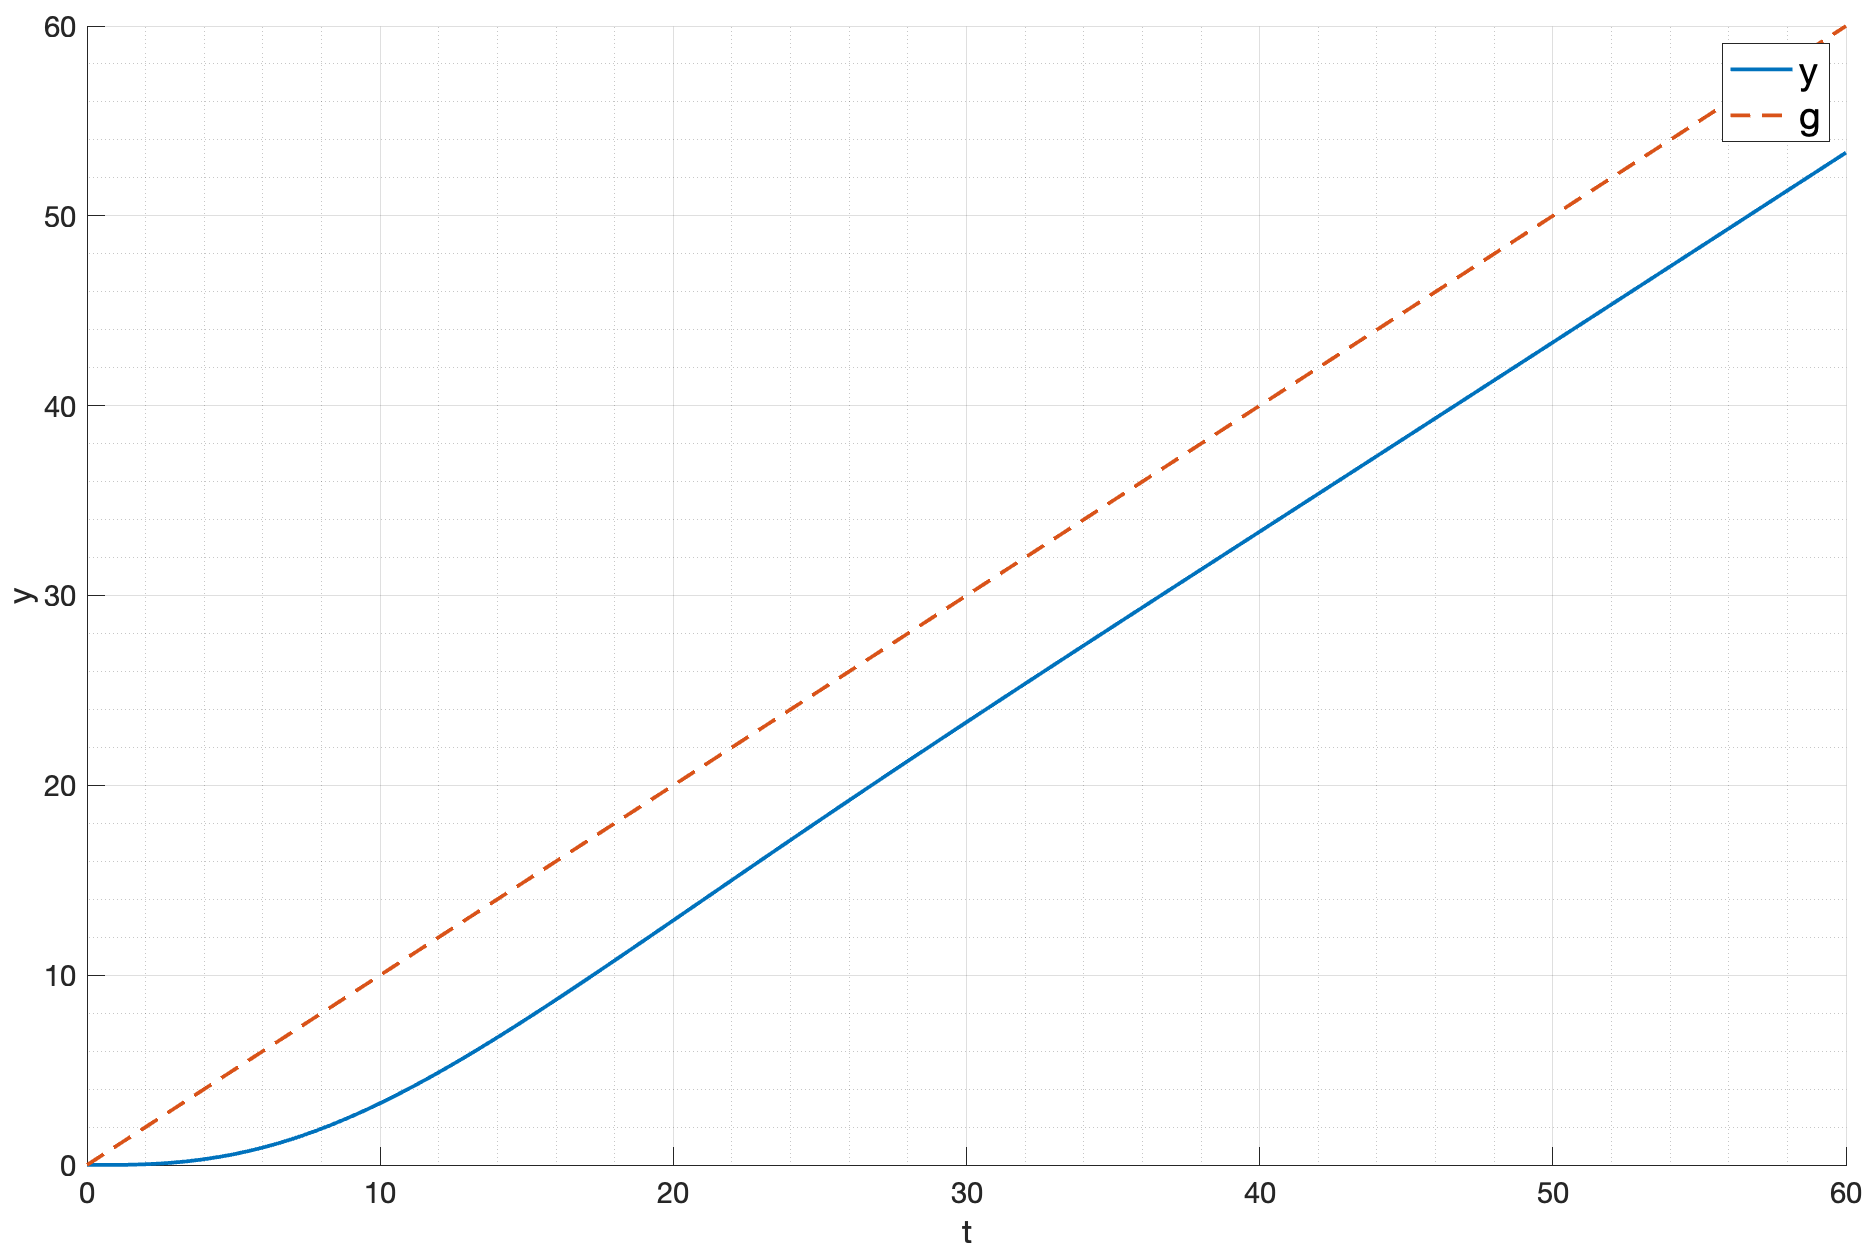
\includegraphics[width=\textwidth]{"media/plots/task4_out4.png"}
%     \caption{Моделирование системы с I регулятором ($k = 0.1$) ($u(t) = Vt$)}
%     \label{fig:task4_out4}
% \end{figure}

% \begin{figure}
%     \centering
%     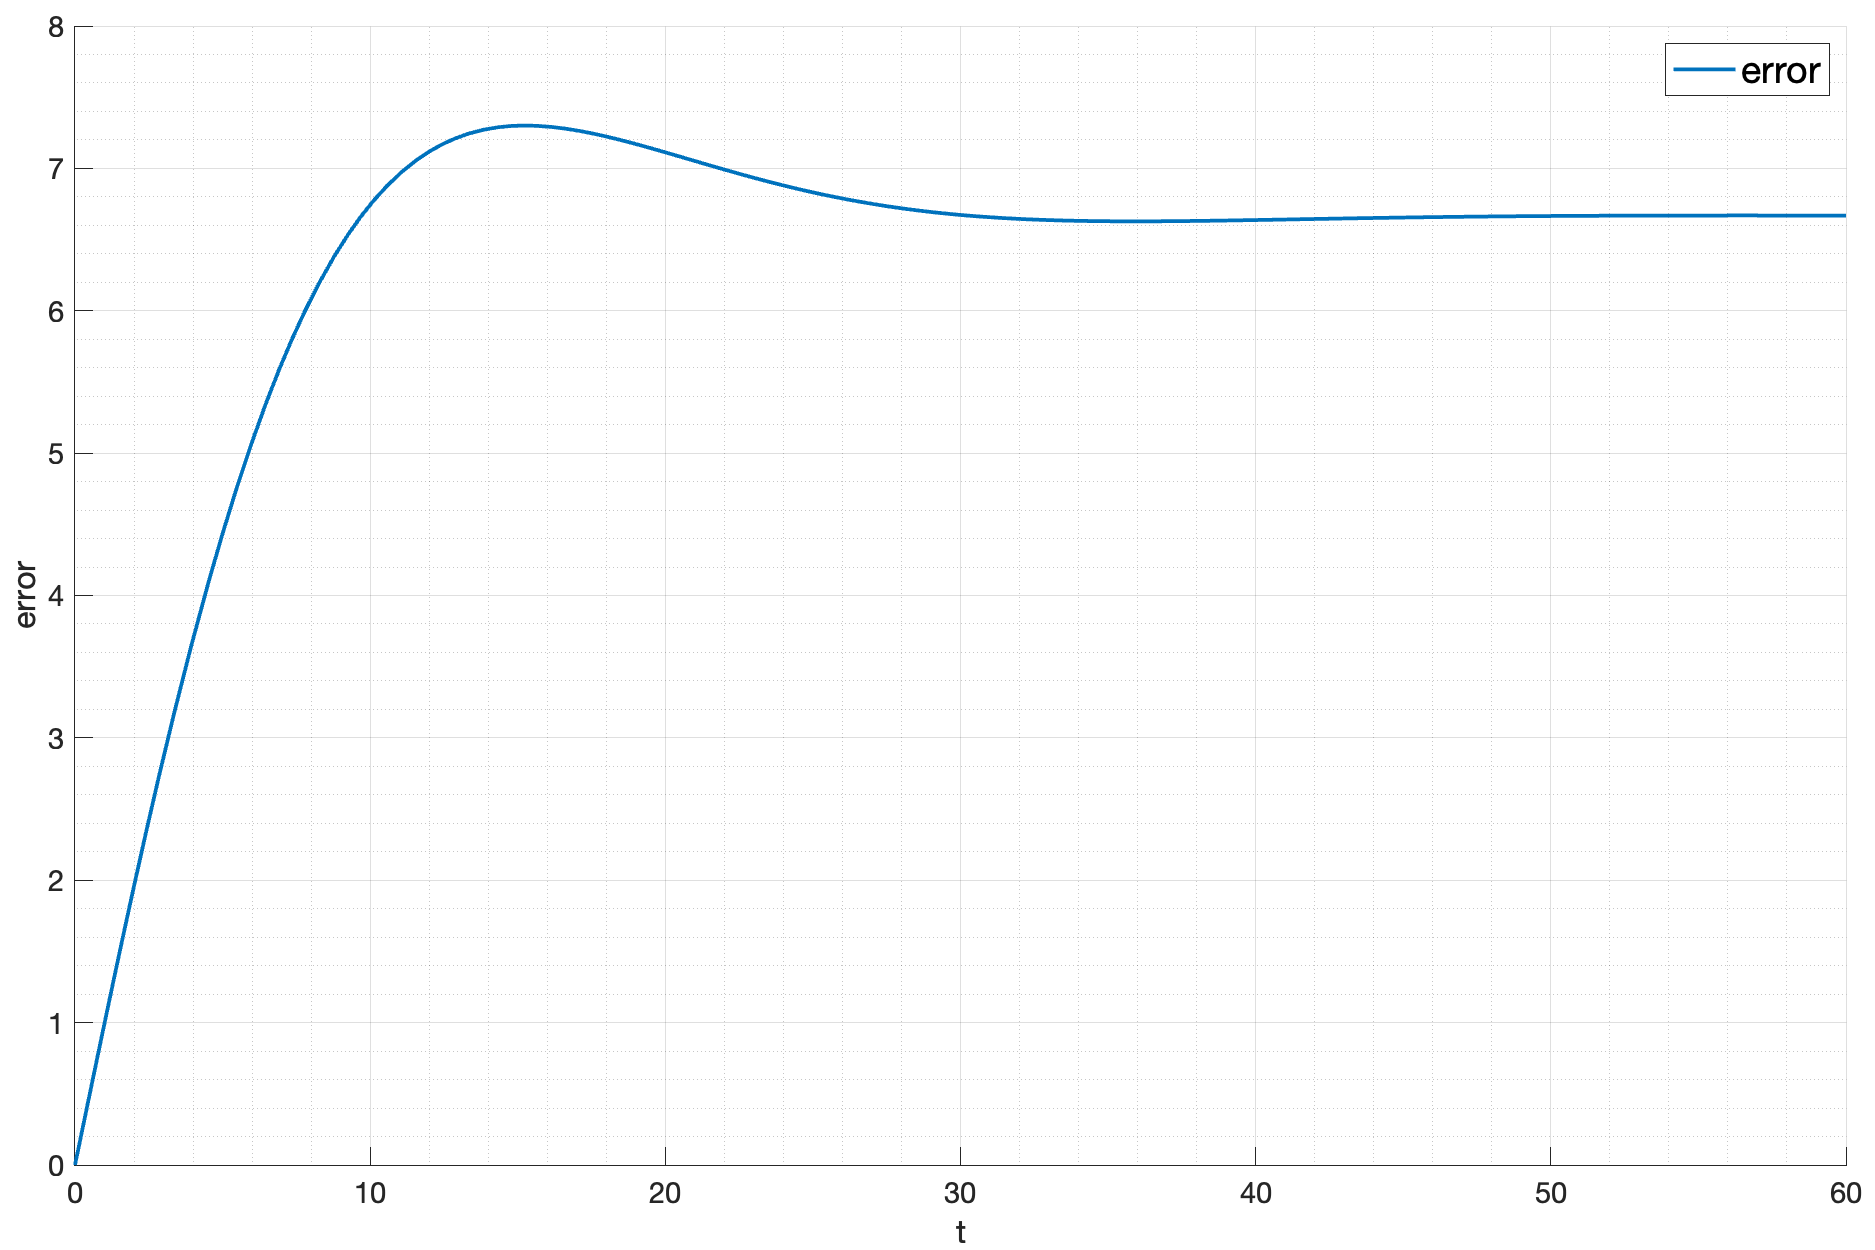
\includegraphics[width=\textwidth]{"media/plots/task4_error4.png"}
%     \caption{График ошибки системы с I регулятором ($k = 0.1$) ($u(t) = Vt$)}
%     \label{fig:task4_error4}
% \end{figure}

% Возьмем $k = 0.3$. Таким образом, согласно теоретическим расчетам, система будет устойчива. Промоделируем (см рис. \ref{fig:task4_out5}).
% График ошибки приведен на рис. \ref{fig:task4_error5}. Теоретическое значение установившегося значения ошибки: $e_{\text{set}} = 2.22$.
% Фактическое значение установившегося значения ошибки: $e_{\text{set}} = 2.22$.

% \begin{figure}[ht!]
%     \centering
%     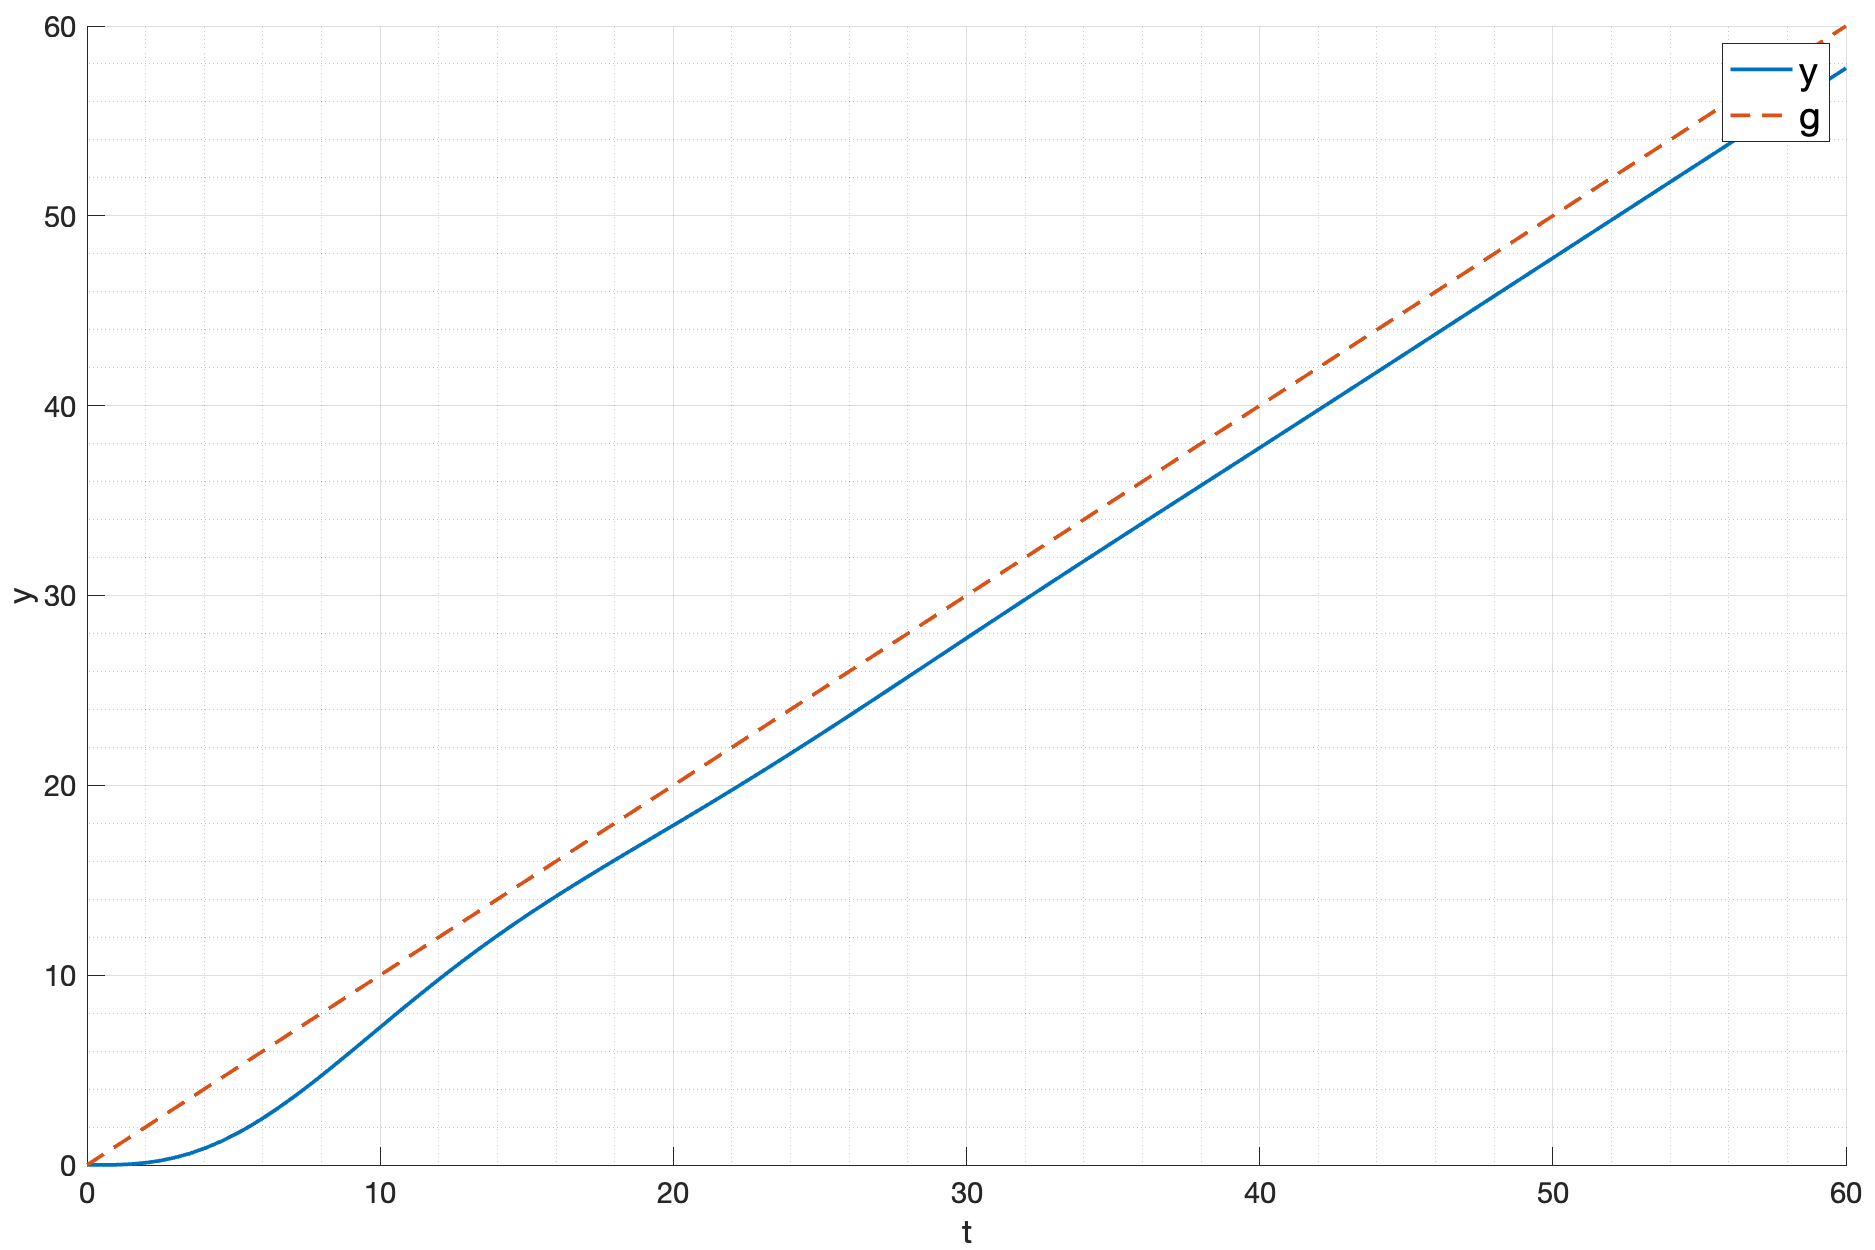
\includegraphics[width=\textwidth]{"media/plots/task4_out5.png"}
%     \caption{Моделирование системы с I регулятором ($k = 0.3$) ($u(t) = Vt$)}
%     \label{fig:task4_out5}
% \end{figure}

% \begin{figure}
%     \centering
%     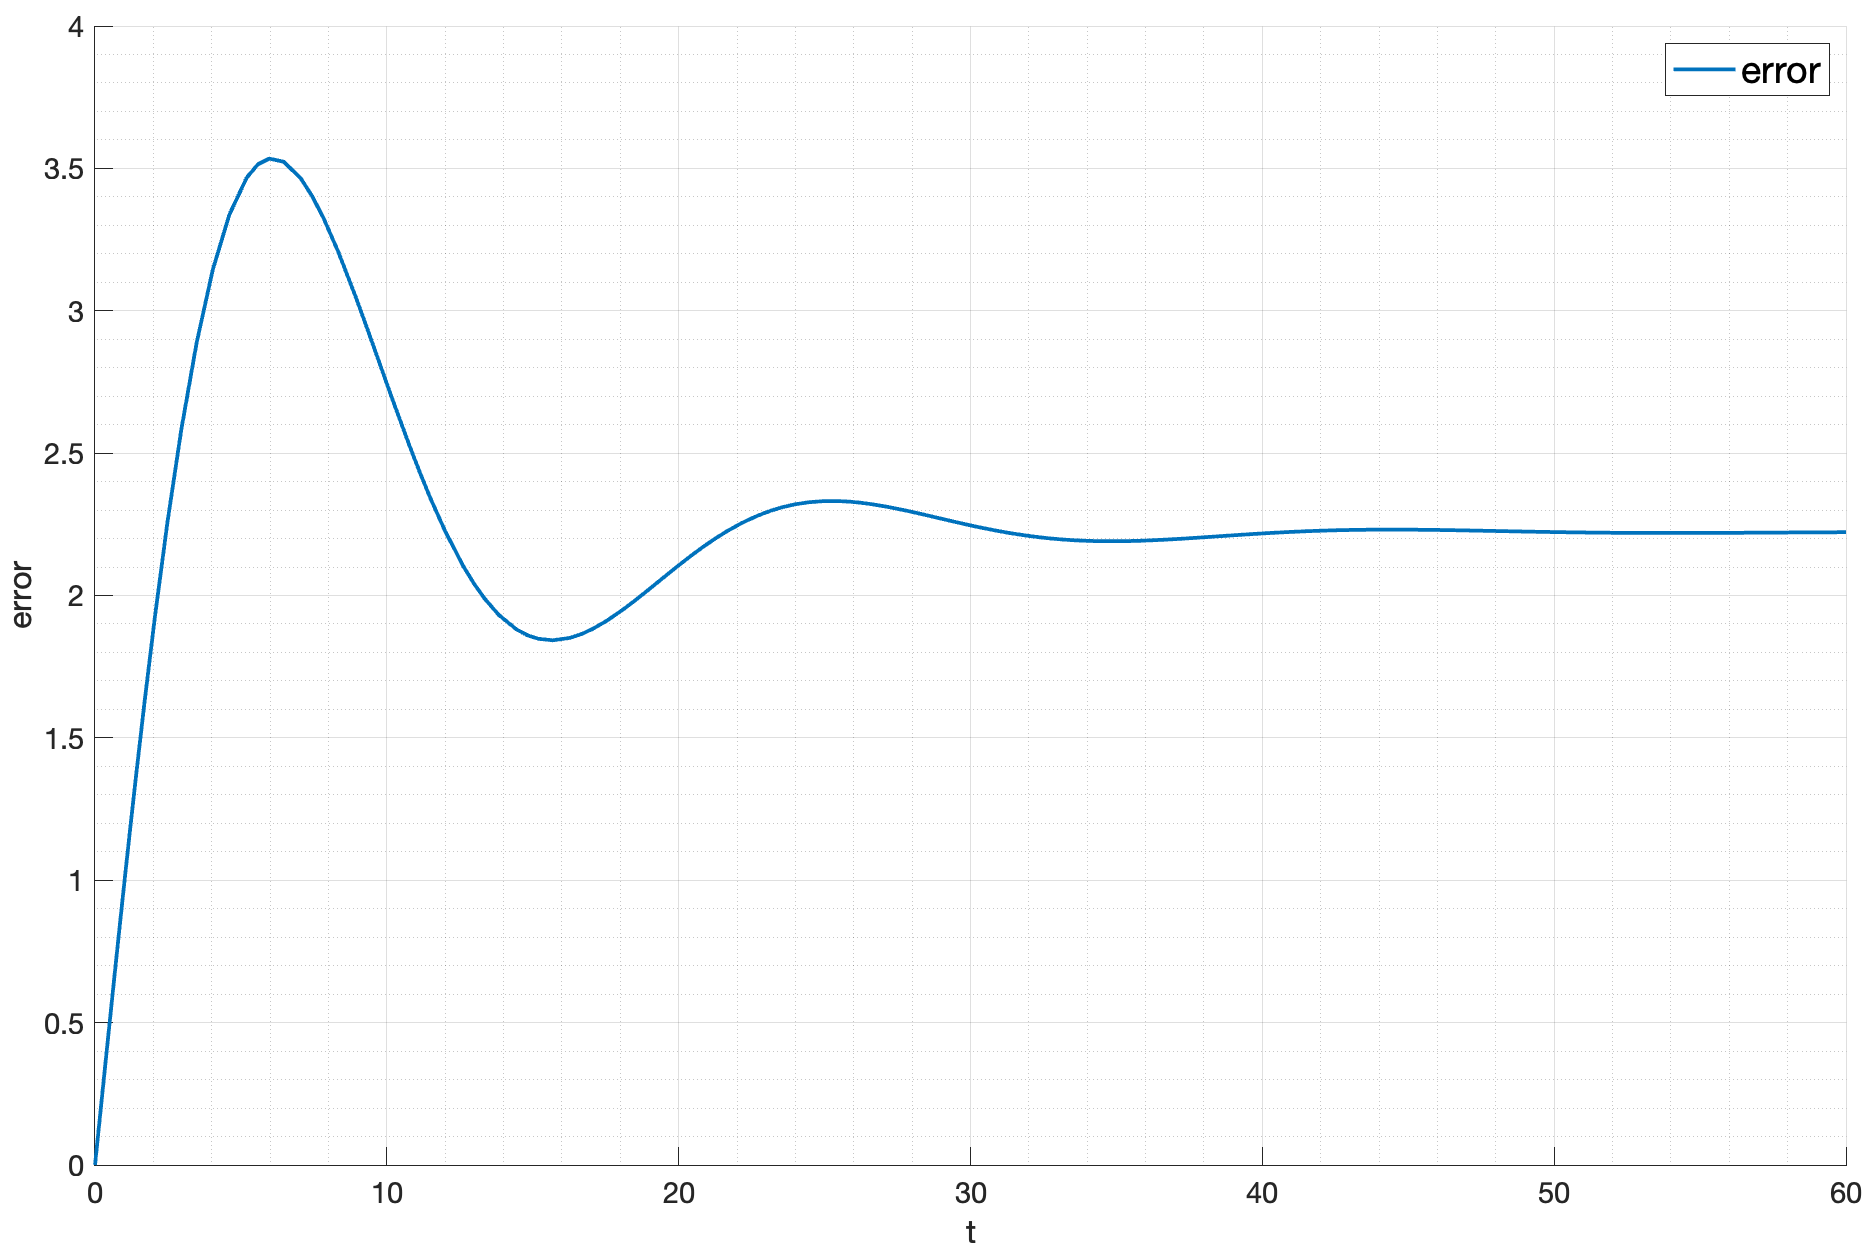
\includegraphics[width=\textwidth]{"media/plots/task4_error5.png"}
%     \caption{График ошибки системы с I регулятором ($k = 0.3$) ($u(t) = Vt$)}
%     \label{fig:task4_error5}
% \end{figure}

% Возьмем $k = 0.5$. Таким образом, согласно теоретическим расчетам, система будет устойчива. Промоделируем (см рис. \ref{fig:task4_out6}).
% График ошибки приведен на рис. \ref{fig:task4_error6}. Теоретическое значение установившегося значения ошибки: $e_{\text{set}} = 1.33$.
% Фактическое значение установившегося значения ошибки: $e_{\text{set}} = 1.33$.

% \begin{figure}[ht!]
%     \centering
%     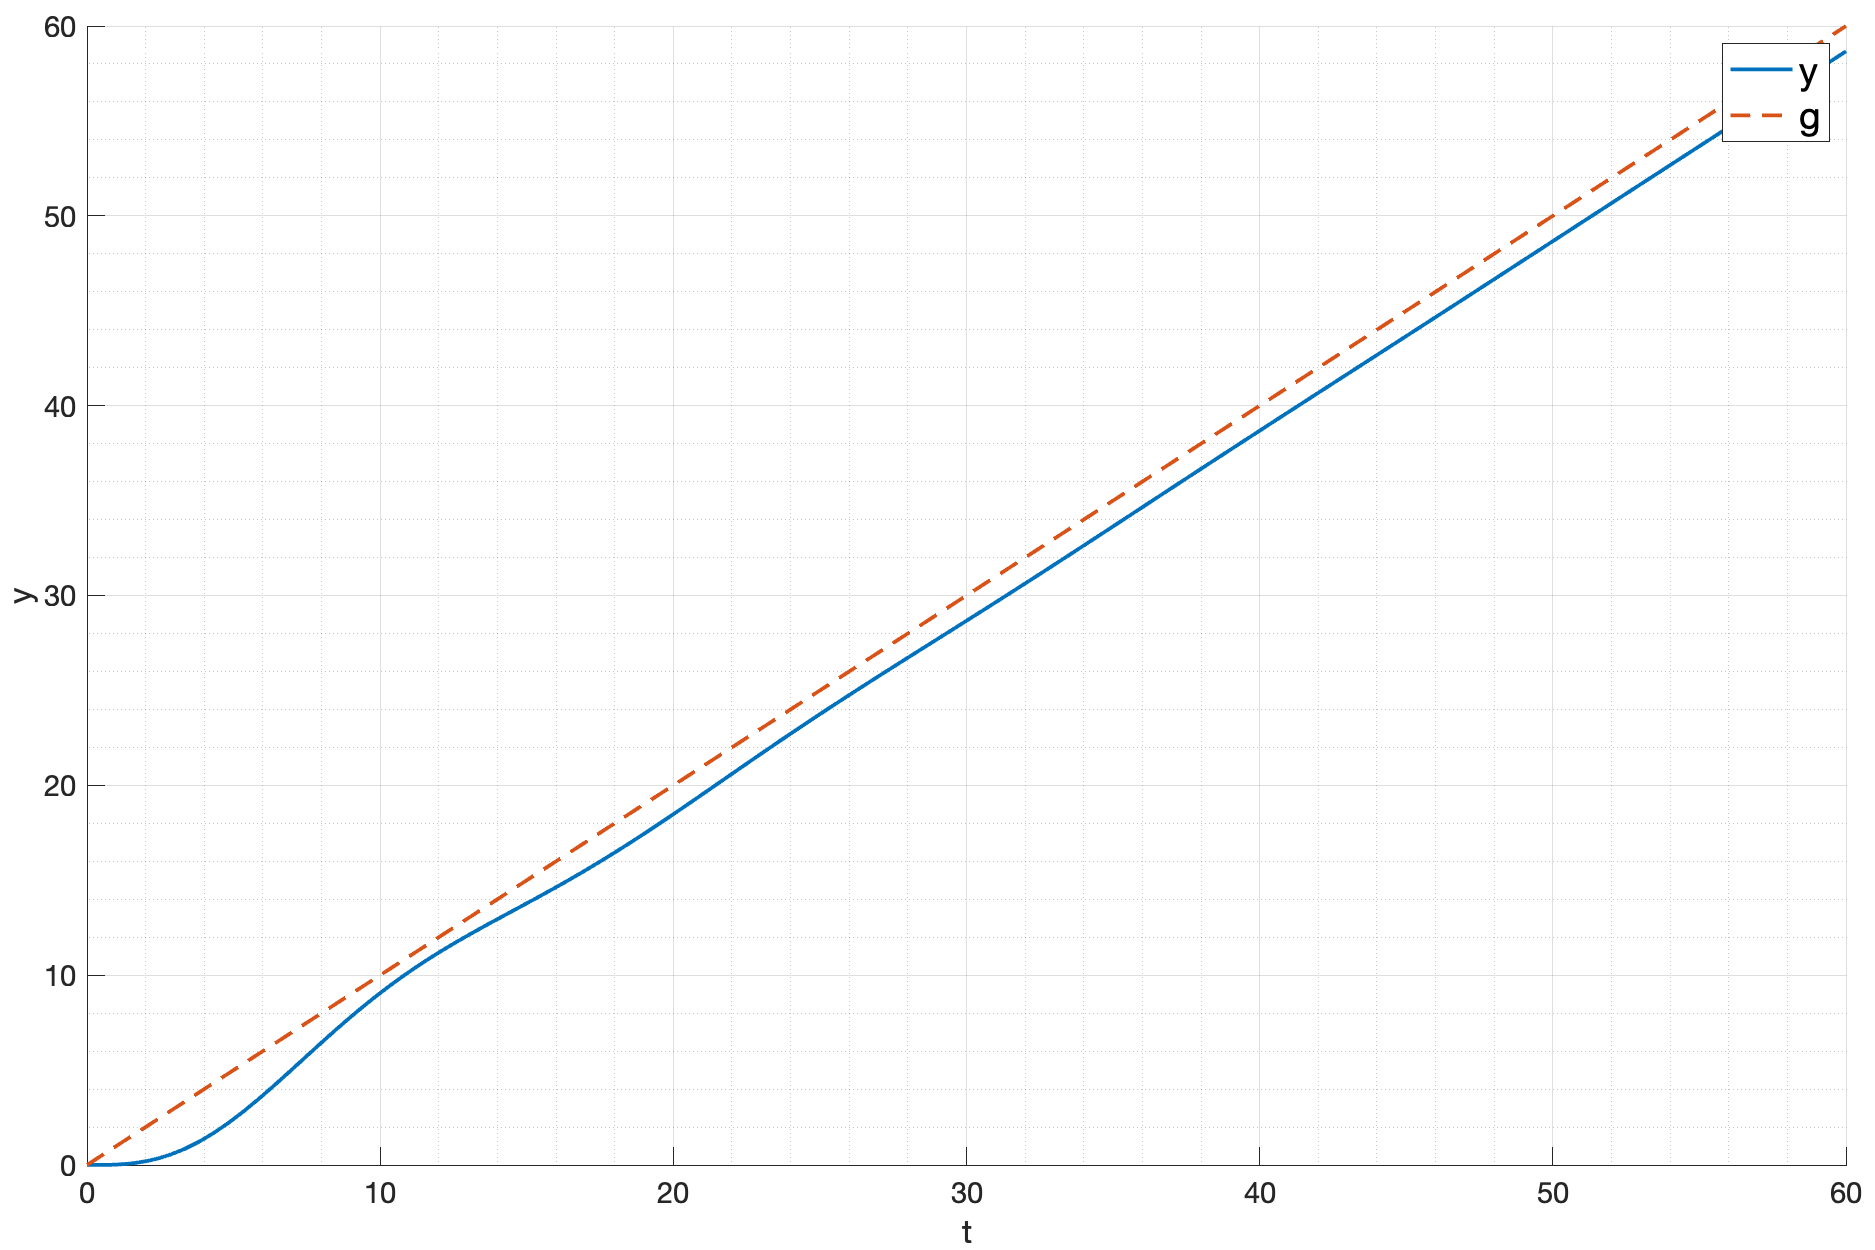
\includegraphics[width=\textwidth]{"media/plots/task4_out6.png"}
%     \caption{Моделирование системы с I регулятором ($k = 0.5$) ($u(t) = Vt$)}
%     \label{fig:task4_out6}
% \end{figure}

% \begin{figure}
%     \centering
%     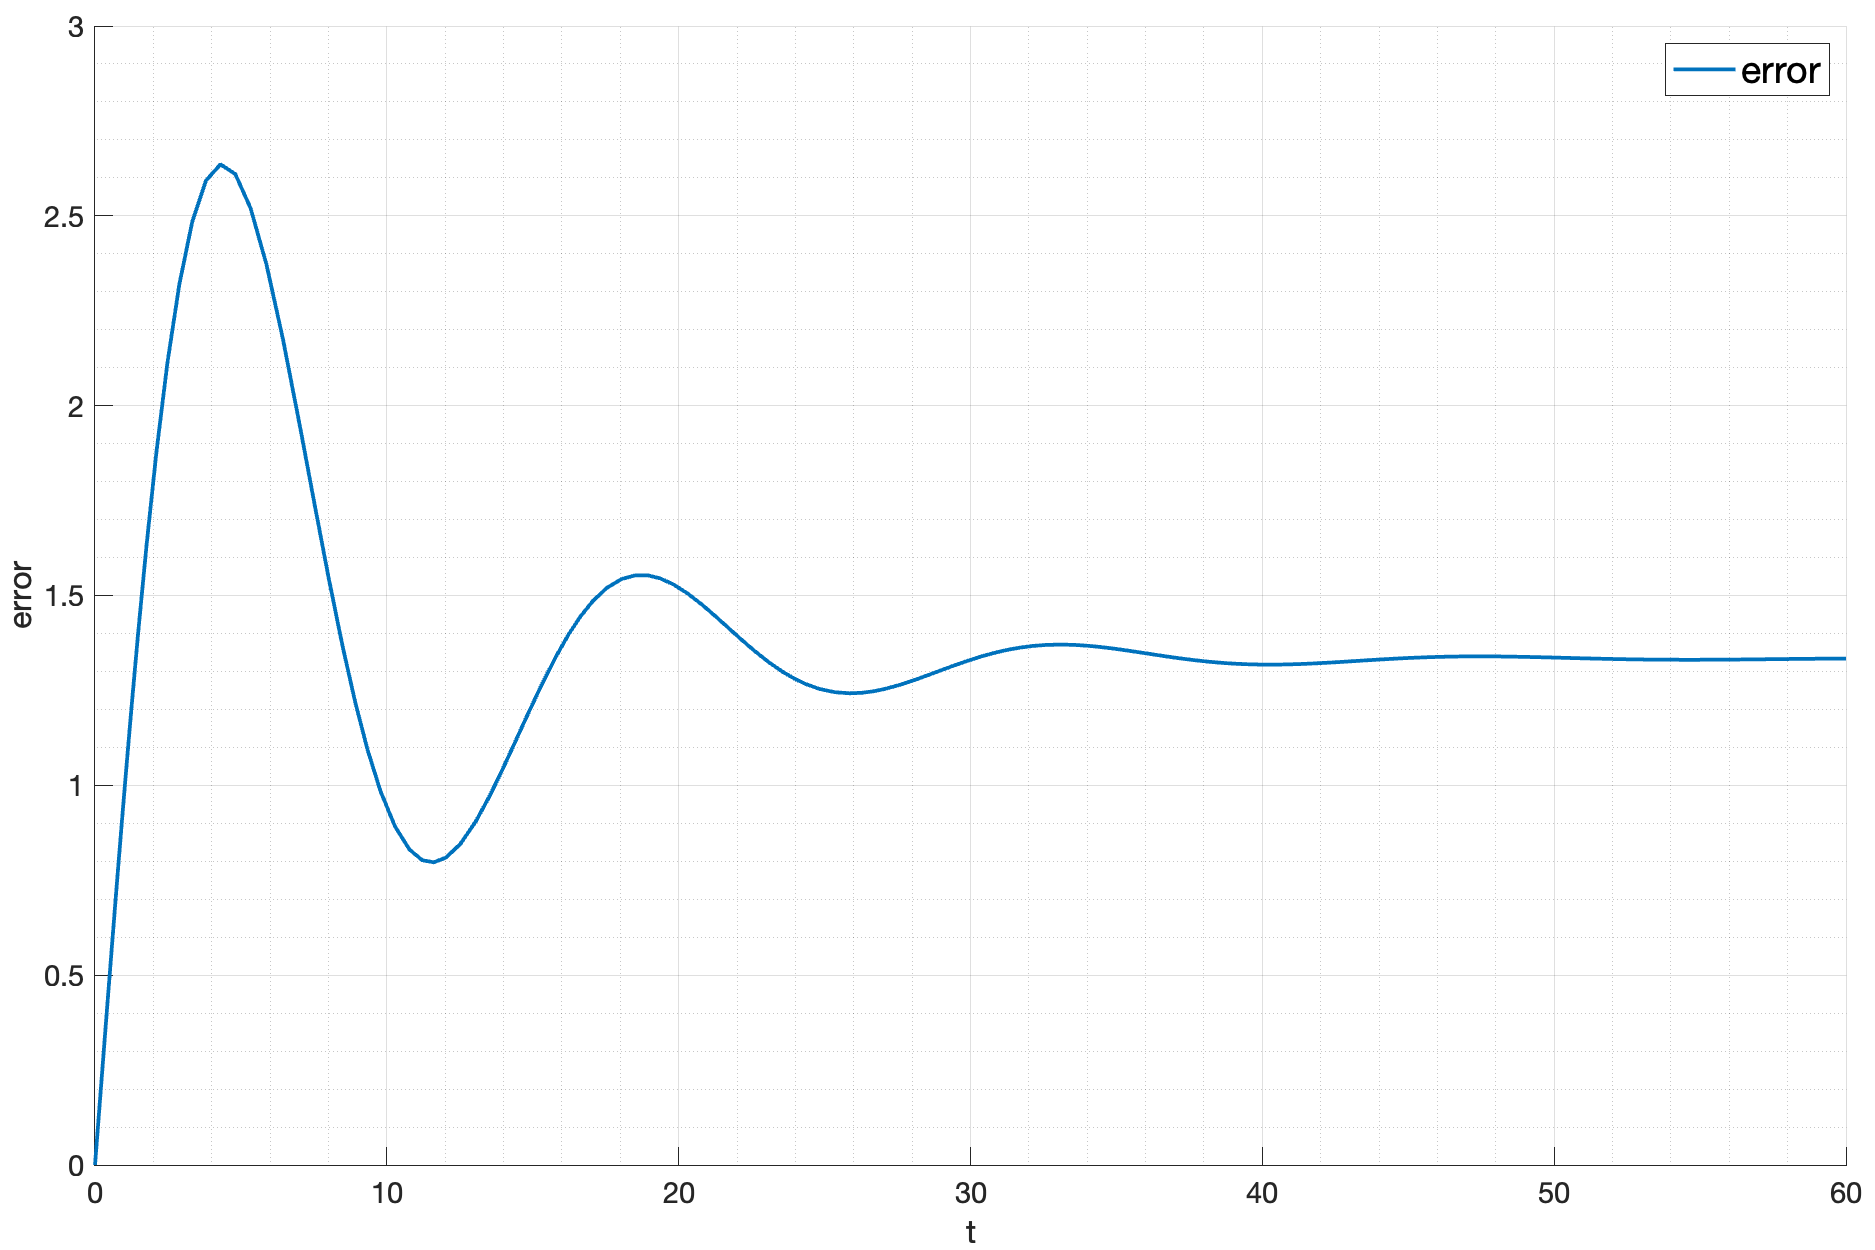
\includegraphics[width=\textwidth]{"media/plots/task4_error6.png"}
%     \caption{График ошибки системы с I регулятором ($k = 0.5$) ($u(t) = Vt$)}
%     \label{fig:task4_error6}
% \end{figure}

Видно, что во всех трех случаях система устойчива и ошибки стремятся к теоретическим значениям. 

\subsection{Квадратичное входное воздействие}
Рассмотрим систему с квадратичным входным воздействием:
\begin{equation}
    u(t) = \frac{at^2}{2}
\end{equation}
Найдем образ Лапласа входного воздействия:
\begin{equation}
    L\{u\} = \frac{a}{s^3}
\end{equation}
Найдем образ Лапласа ошибки:
\begin{equation}
    E = W_{u\rightarrow e}(s)L\{u\} = \frac{s(s^2 + 7.5s + 2)}{s(s^2 + 7.5s + 2) + 3k}\frac{a}{s^3} = \frac{a(s^2 + 7.5s + 2)}{s^2(s(s^2 + 7.5s + 2) + 3k)}
\end{equation}
Значение $sE$ имеет нулевые полюса, следовательно, теорема о конечном значении не применима.

Проведем моделирование системы с квадратичным входным воздействием при значениях $k = \{0.1, 0.3, 0.5\}$.
Результаты моделирования приведены на рис. \ref{fig:task4_out3}, \ref{fig:task4_error3}.

\begin{figure}[ht!]
    \centering
    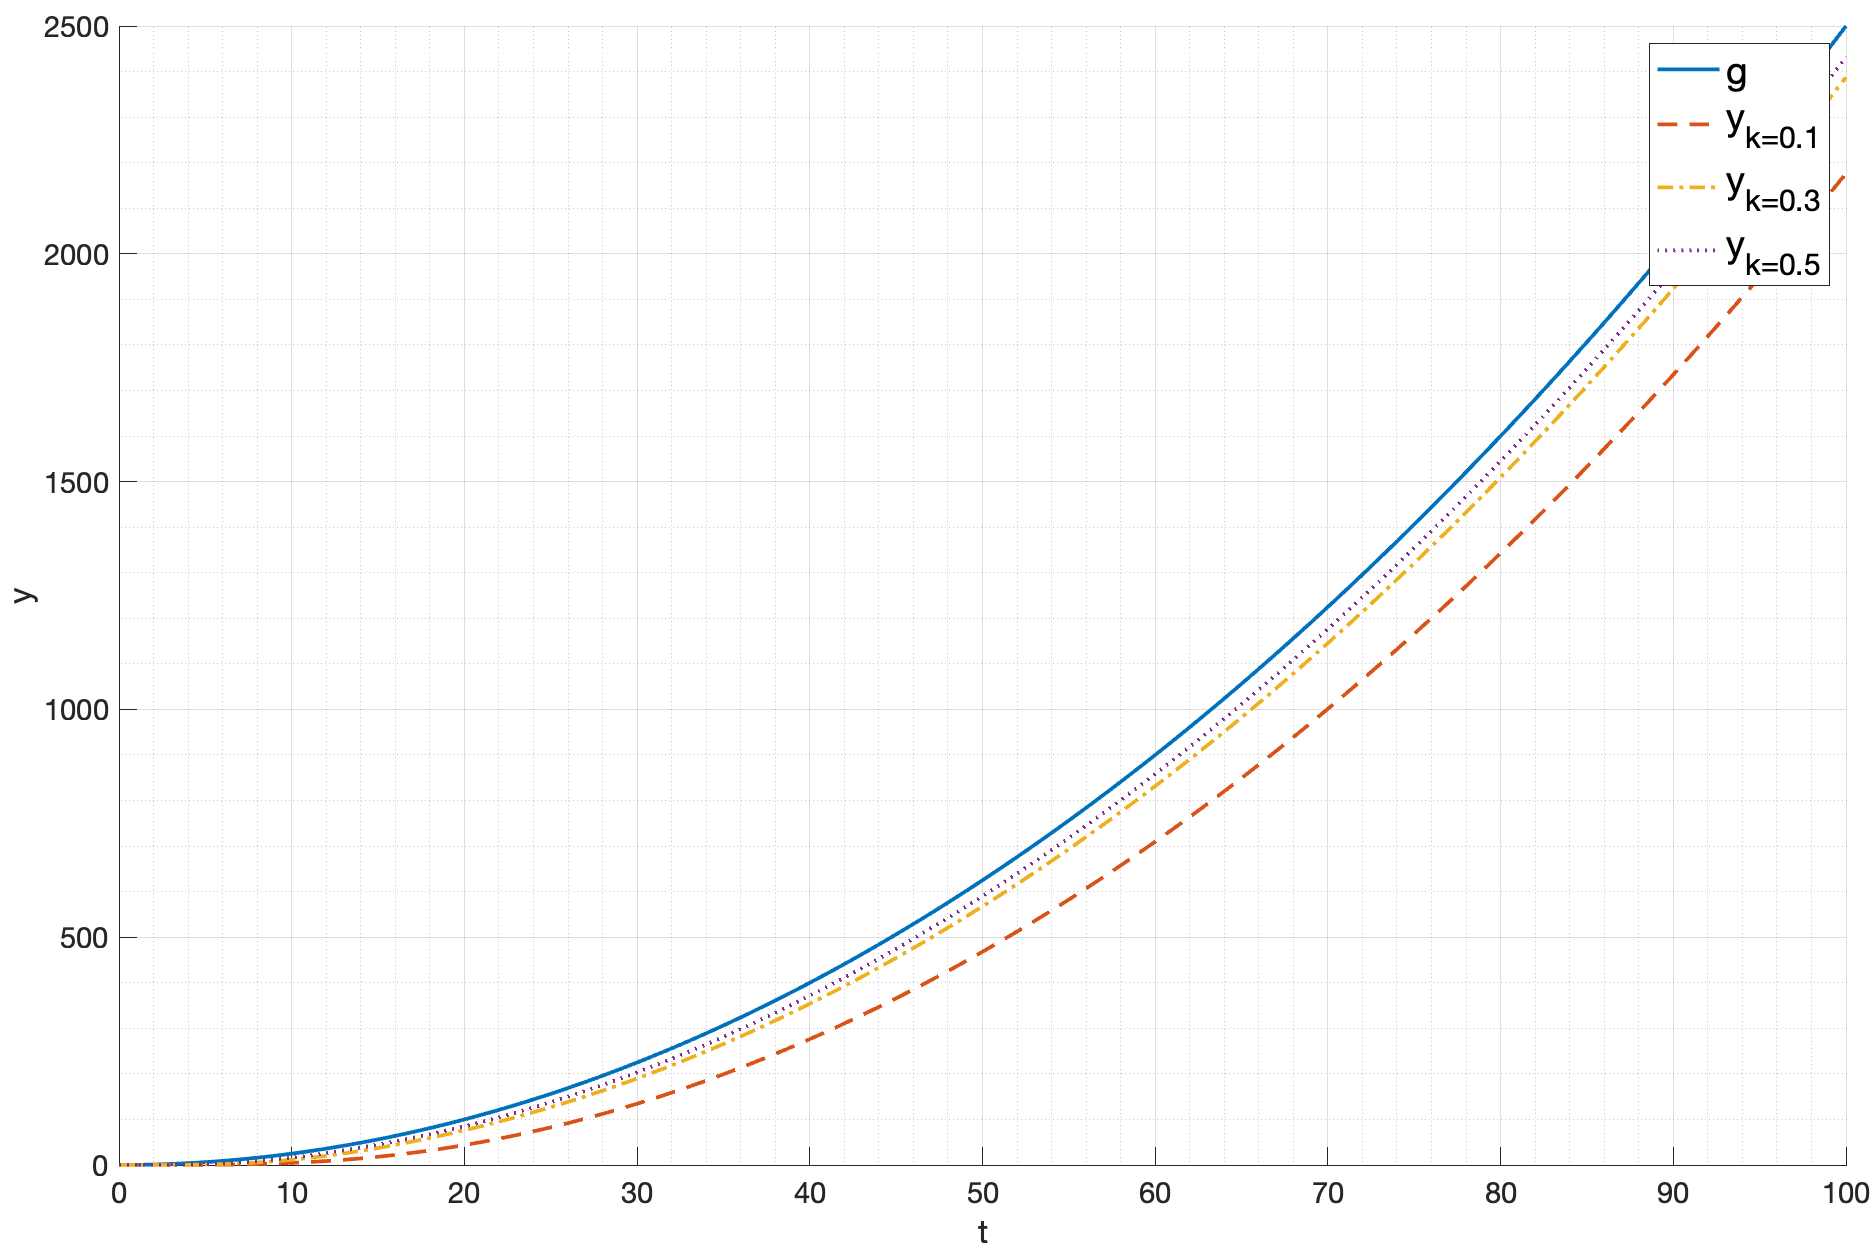
\includegraphics[width=\textwidth]{"media/plots/task4_out3.png"}
    \caption{Моделирование системы с I регулятором ($u(t) = \frac{at^2}{2}$)}
    \label{fig:task4_out3}
\end{figure}

\begin{figure}[ht!]
    \centering
    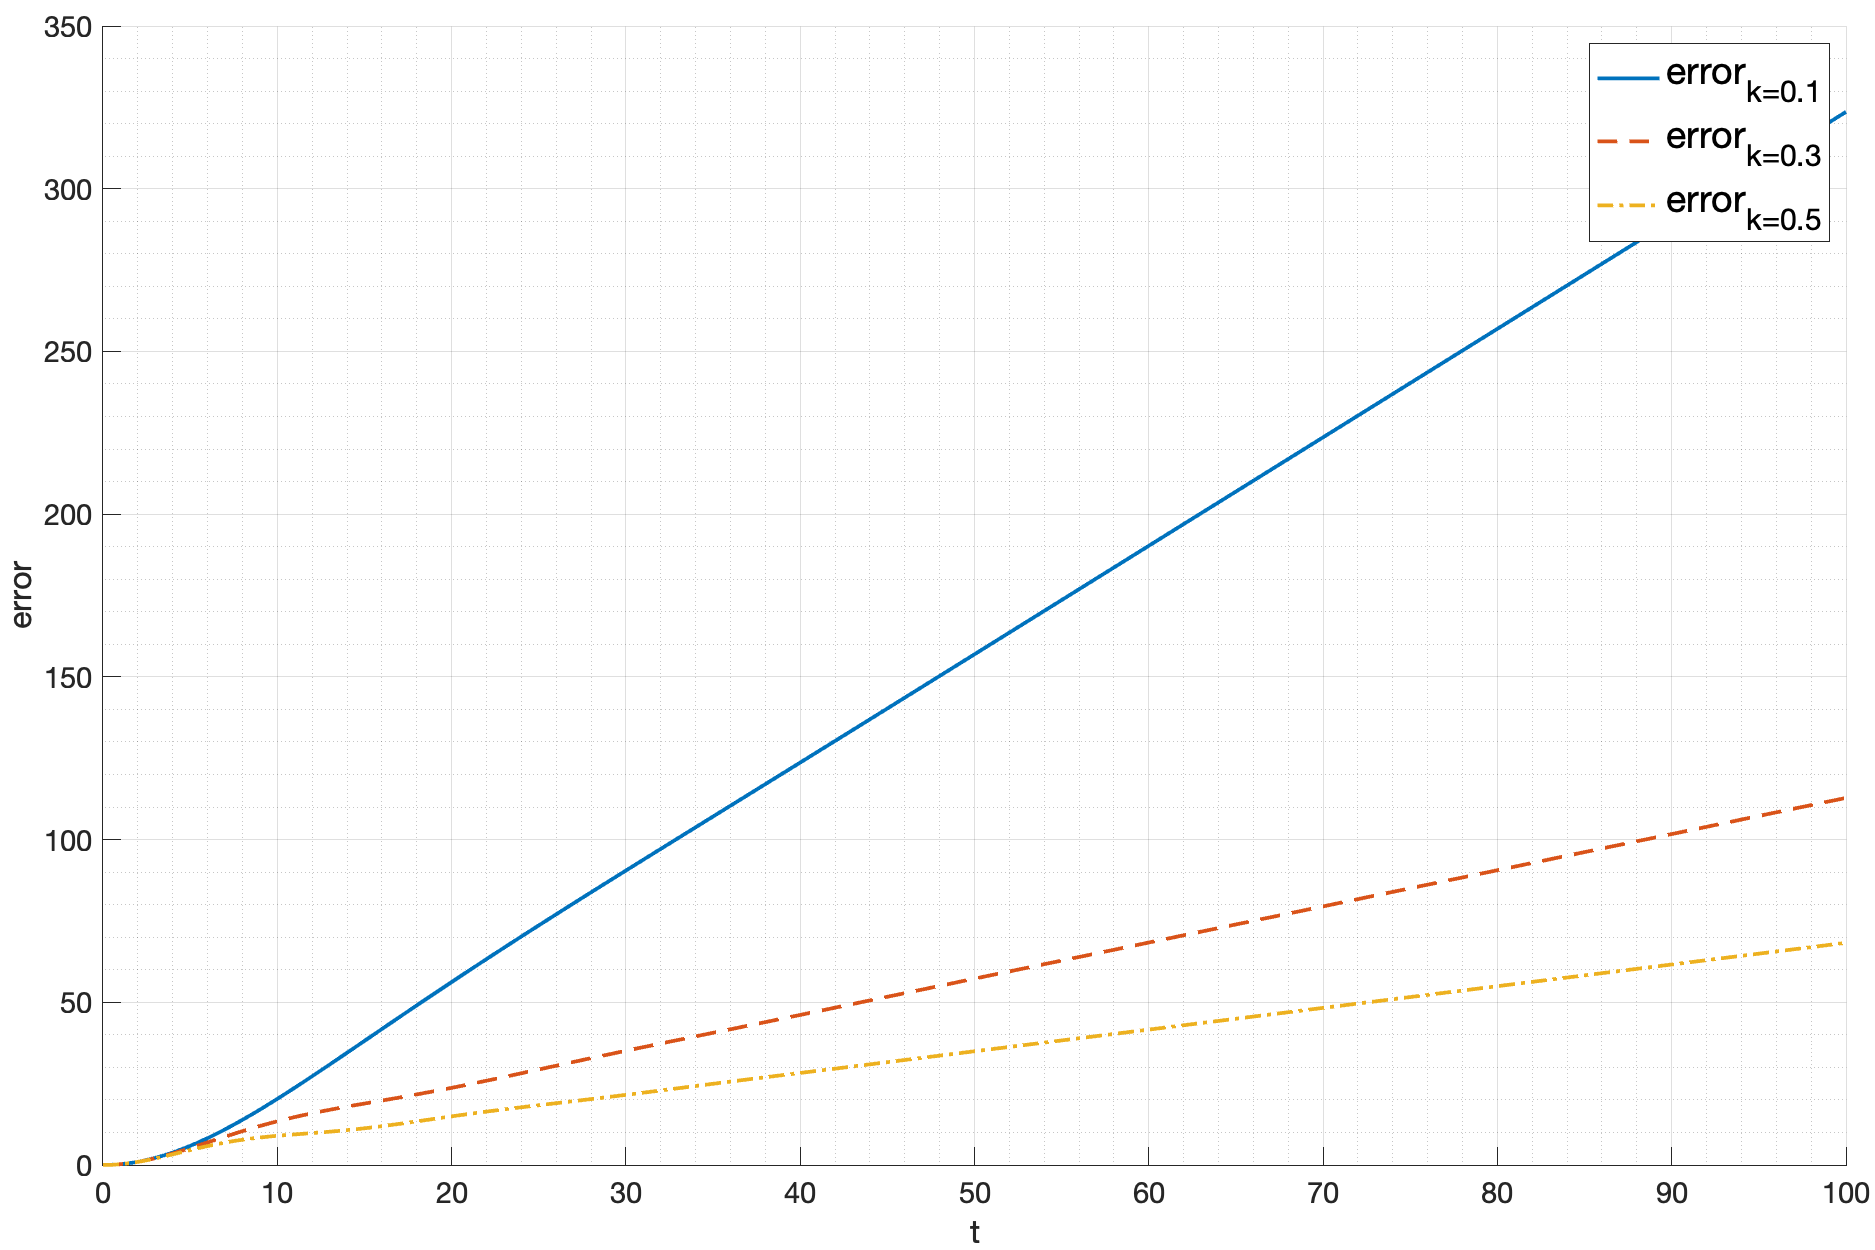
\includegraphics[width=\textwidth]{"media/plots/task4_error3.png"}
    \caption{График ошибки системы с I регулятором ($u(t) = \frac{at^2}{2}$)}
    \label{fig:task4_error3}
\end{figure}

% Возьмем $k = 0.1$. Таким образом, согласно теоретическим расчетам, система будет устойчива. Промоделируем (см рис. \ref{fig:task4_out7}).
% График ошибки приведен на рис. \ref{fig:task4_error7}. 

% \begin{figure}[ht!]
%     \centering
%     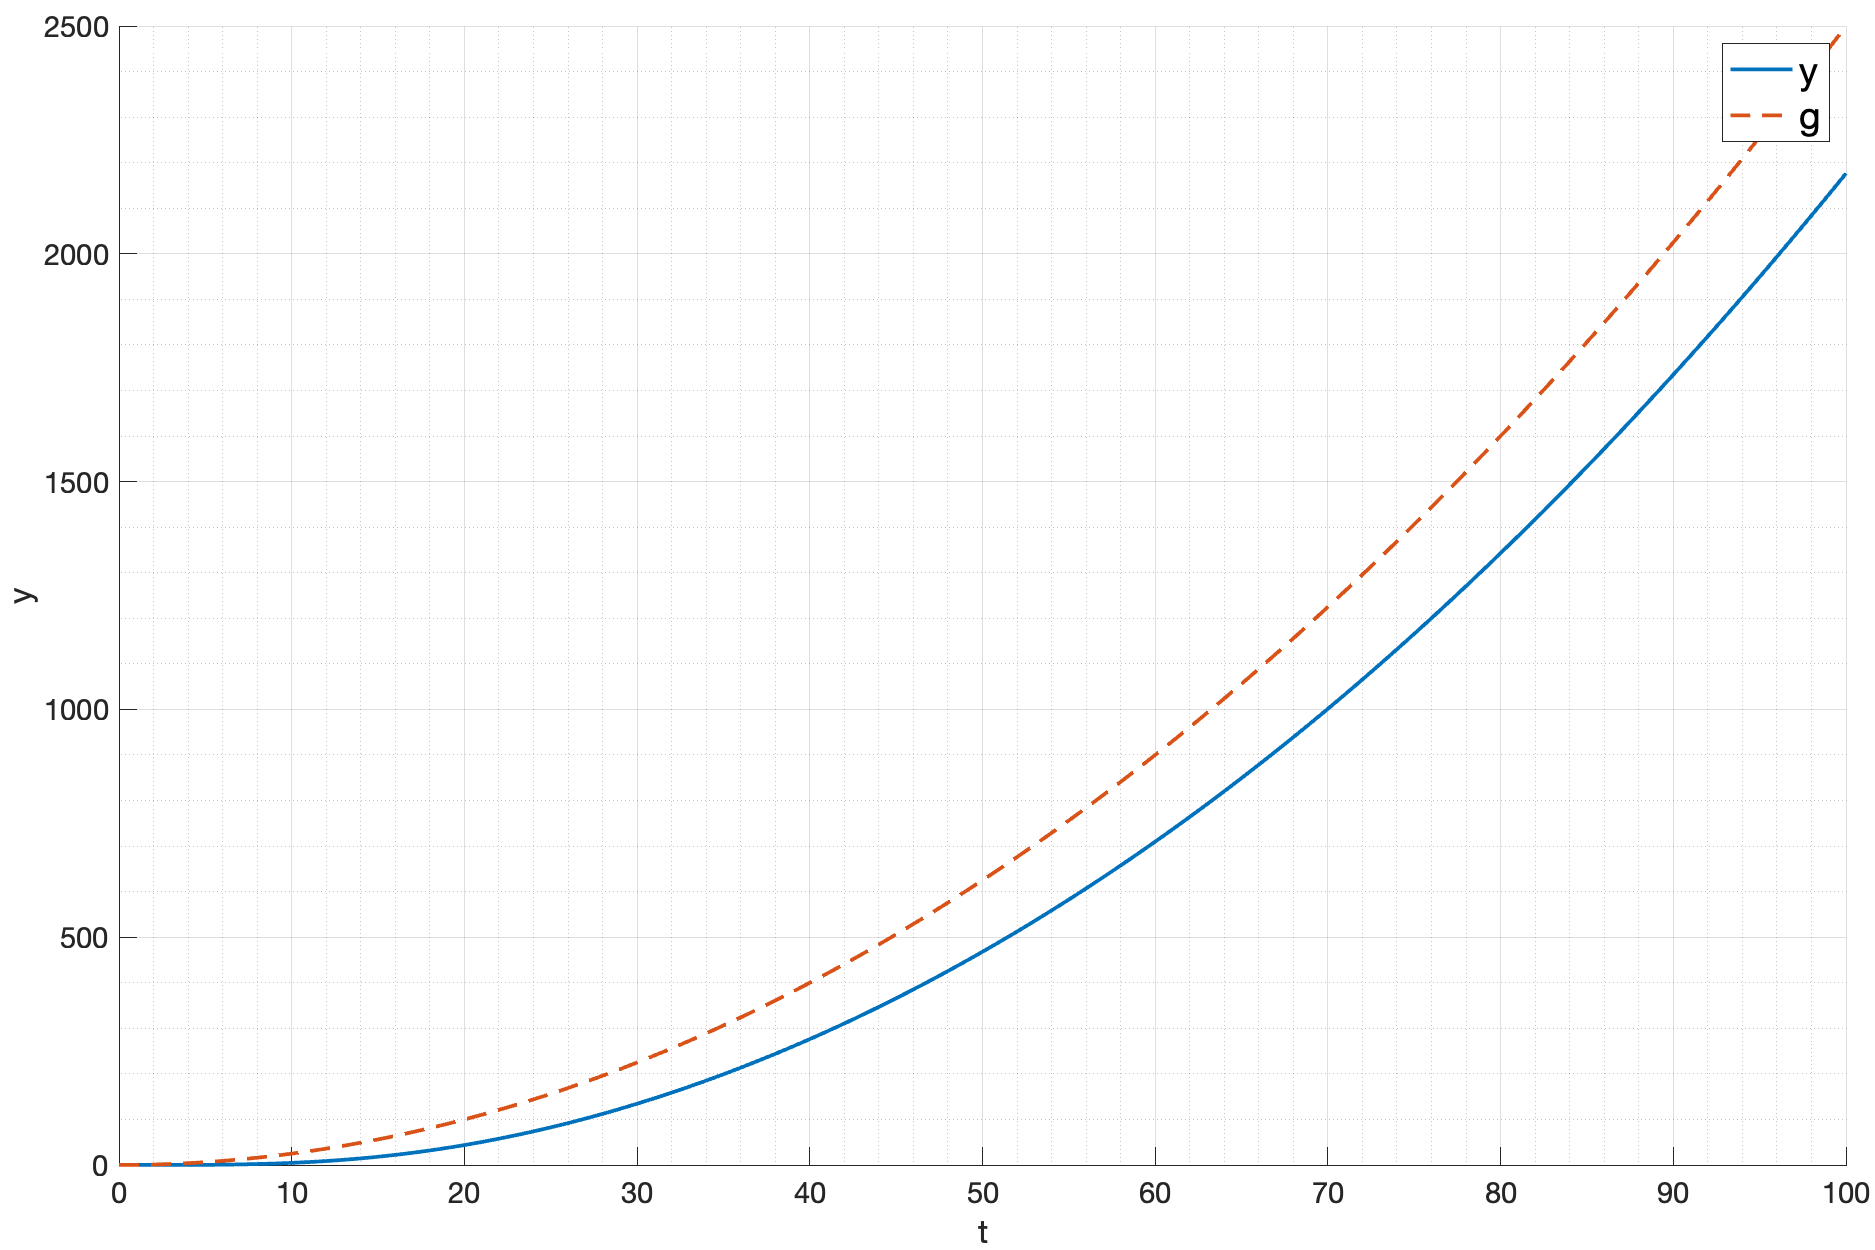
\includegraphics[width=\textwidth]{"media/plots/task4_out7.png"}
%     \caption{Моделирование системы с I регулятором ($k = 0.1$) ($u(t) = \frac{at^2}{2}$)}
%     \label{fig:task4_out7}
% \end{figure}

% \begin{figure}
%     \centering
%     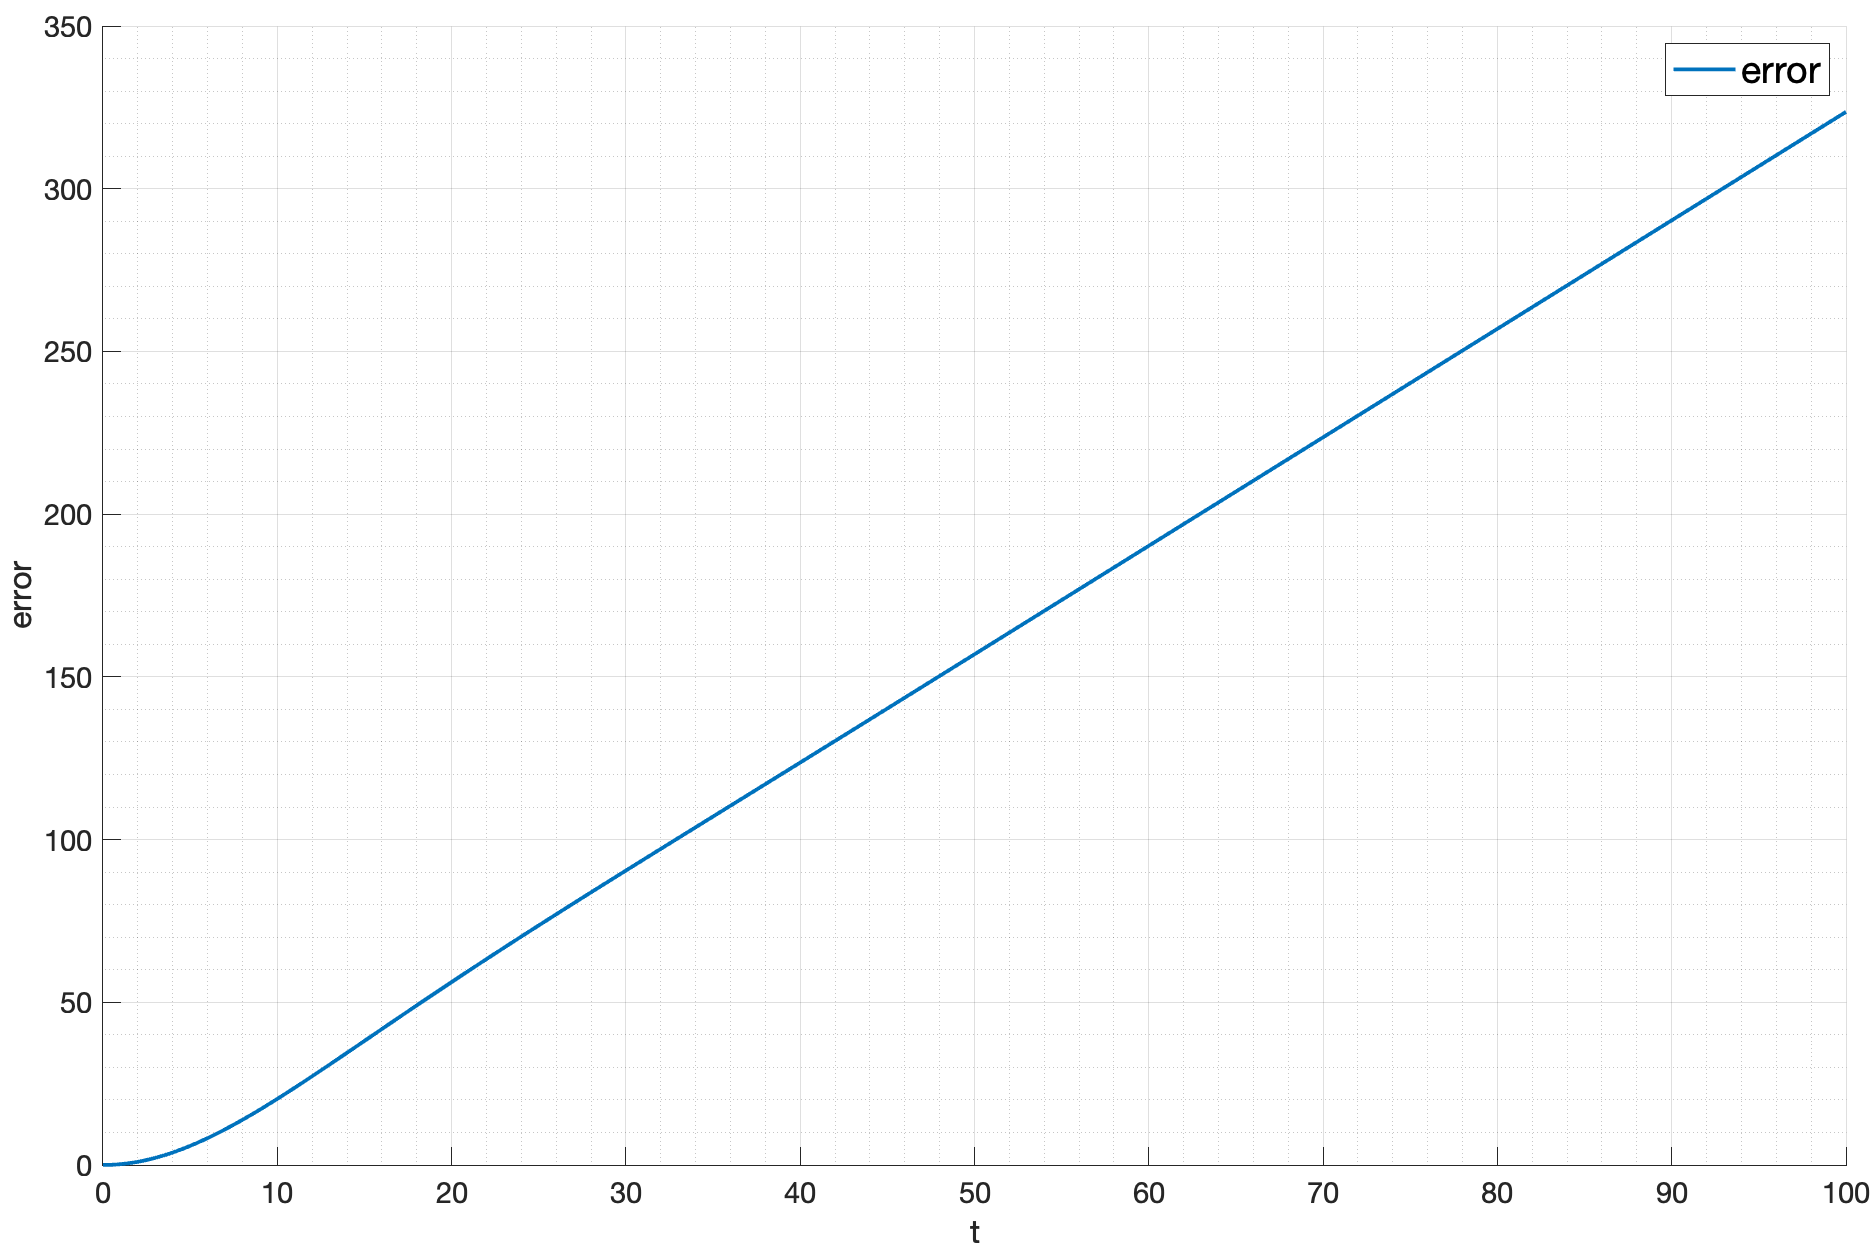
\includegraphics[width=\textwidth]{"media/plots/task4_error7.png"}
%     \caption{График ошибки системы с I регулятором ($k = 0.1$) ($u(t) = \frac{at^2}{2}$)}
%     \label{fig:task4_error7}
% \end{figure}

% Возьмем $k = 0.3$. Таким образом, согласно теоретическим расчетам, система будет устойчива. Промоделируем (см рис. \ref{fig:task4_out8}).
% График ошибки приведен на рис. \ref{fig:task4_error8}. 

% \begin{figure}[ht!]
%     \centering
%     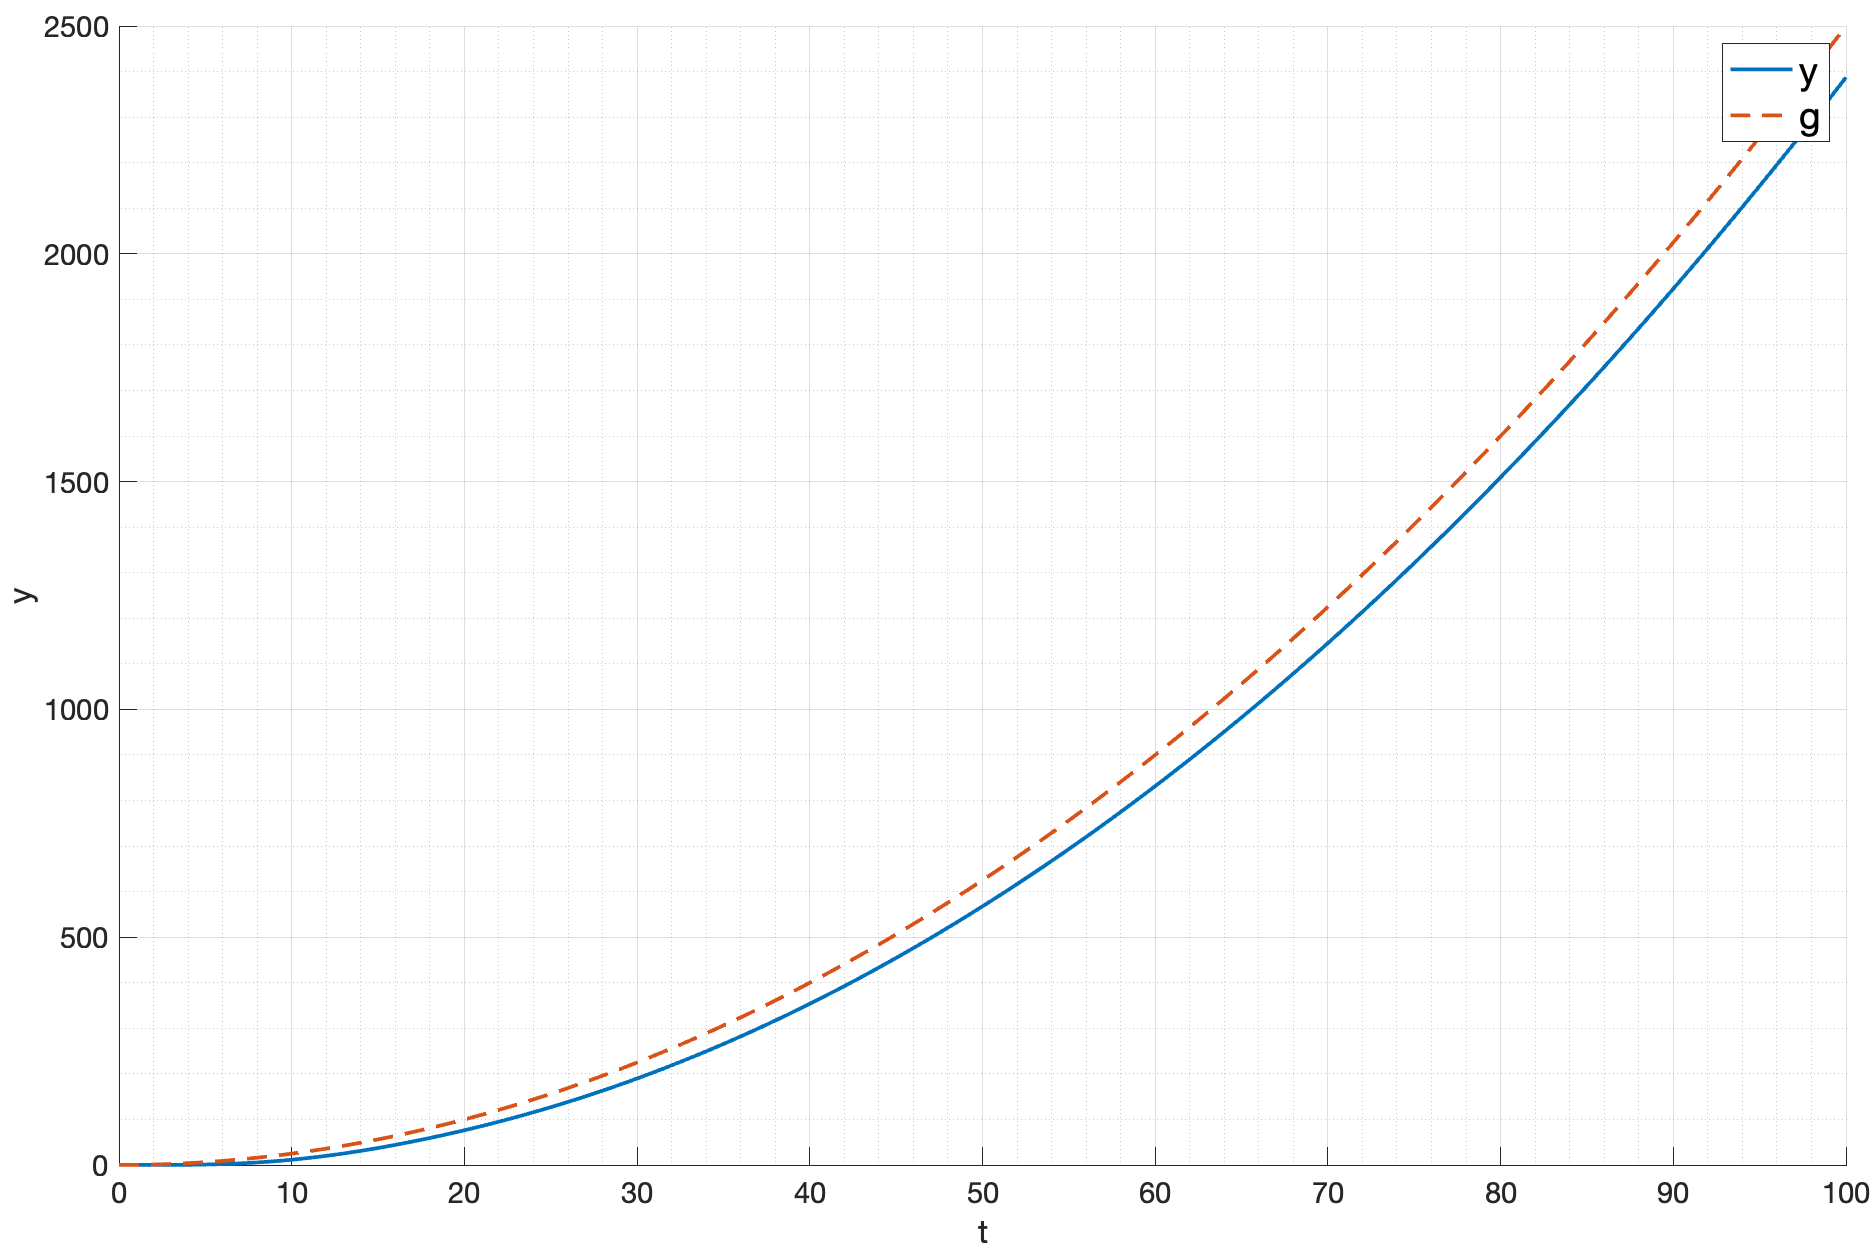
\includegraphics[width=\textwidth]{"media/plots/task4_out8.png"}
%     \caption{Моделирование системы с I регулятором ($k = 0.3$) ($u(t) = \frac{at^2}{2}$)}
%     \label{fig:task4_out8}
% \end{figure}

% \begin{figure}
%     \centering
%     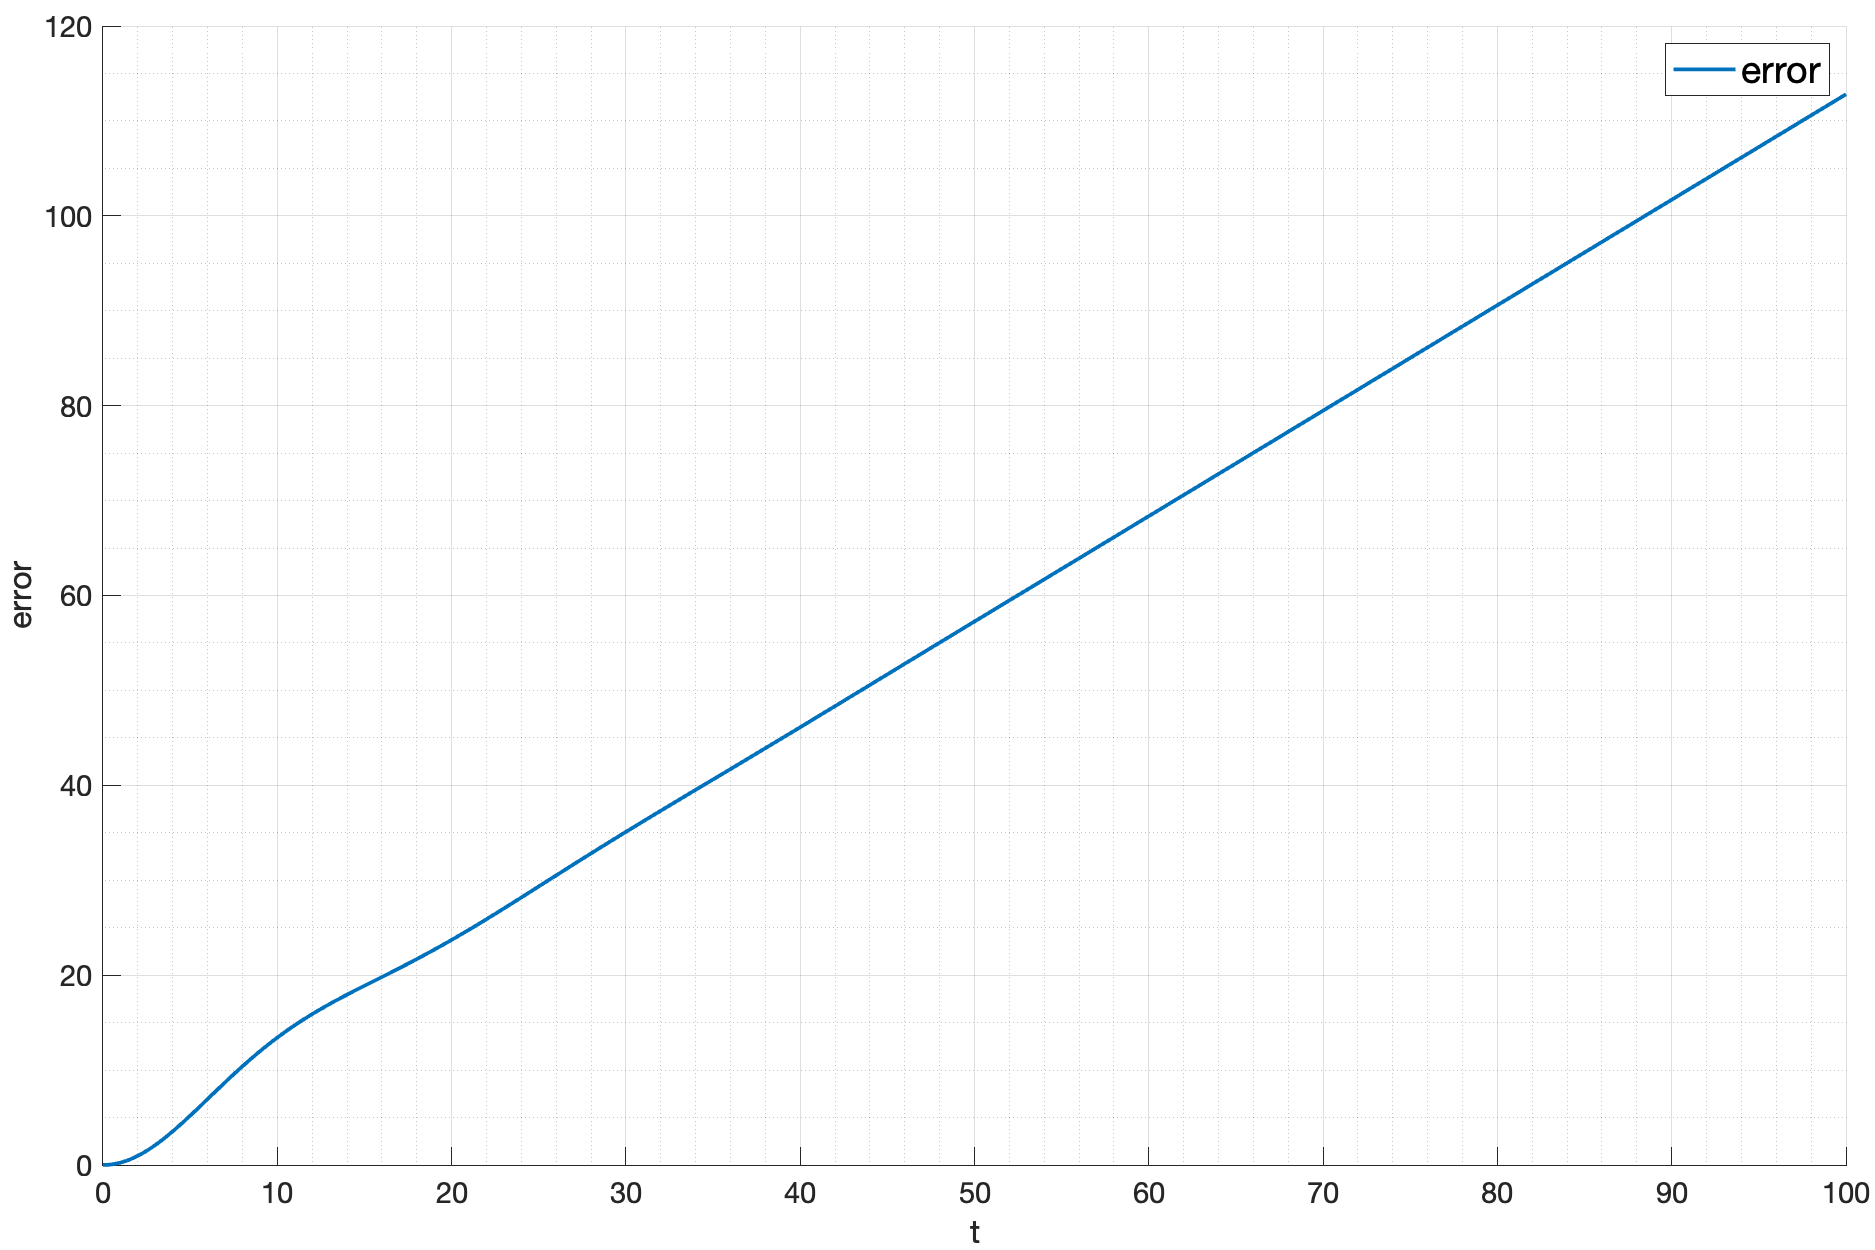
\includegraphics[width=\textwidth]{"media/plots/task4_error8.png"}
%     \caption{График ошибки системы с I регулятором ($k = 0.3$) ($u(t) = \frac{at^2}{2}$)}
%     \label{fig:task4_error8}
% \end{figure}

% Возьмем $k = 0.5$. Таким образом, согласно теоретическим расчетам, система будет устойчива. Промоделируем (см рис. \ref{fig:task4_out9}).
% График ошибки приведен на рис. \ref{fig:task4_error9}. 

% \begin{figure}[ht!]
%     \centering
%     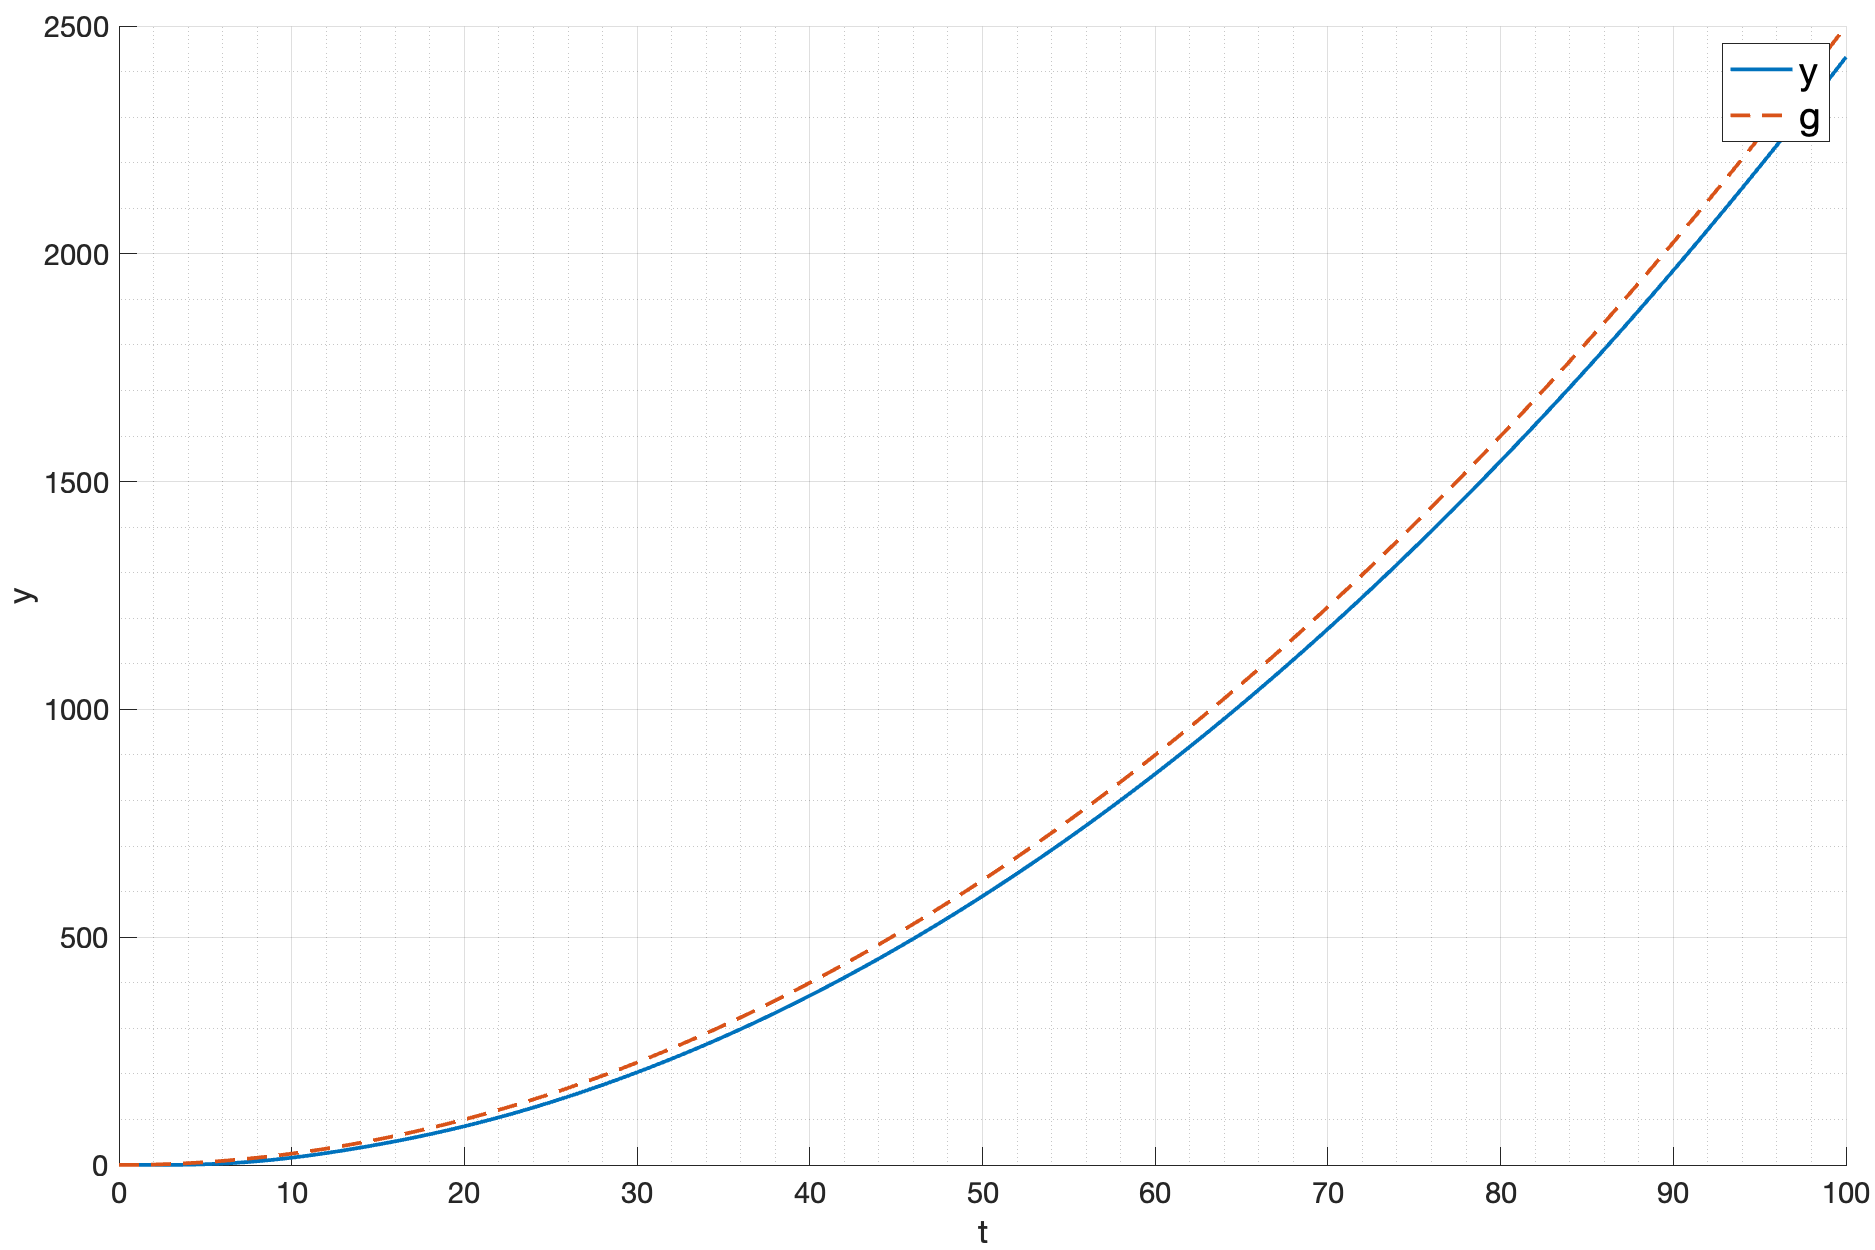
\includegraphics[width=\textwidth]{"media/plots/task4_out9.png"}
%     \caption{Моделирование системы с I регулятором ($k = 0.5$) ($u(t) = \frac{at^2}{2}$)}
%     \label{fig:task4_out9}
% \end{figure}

% \begin{figure}
%     \centering
%     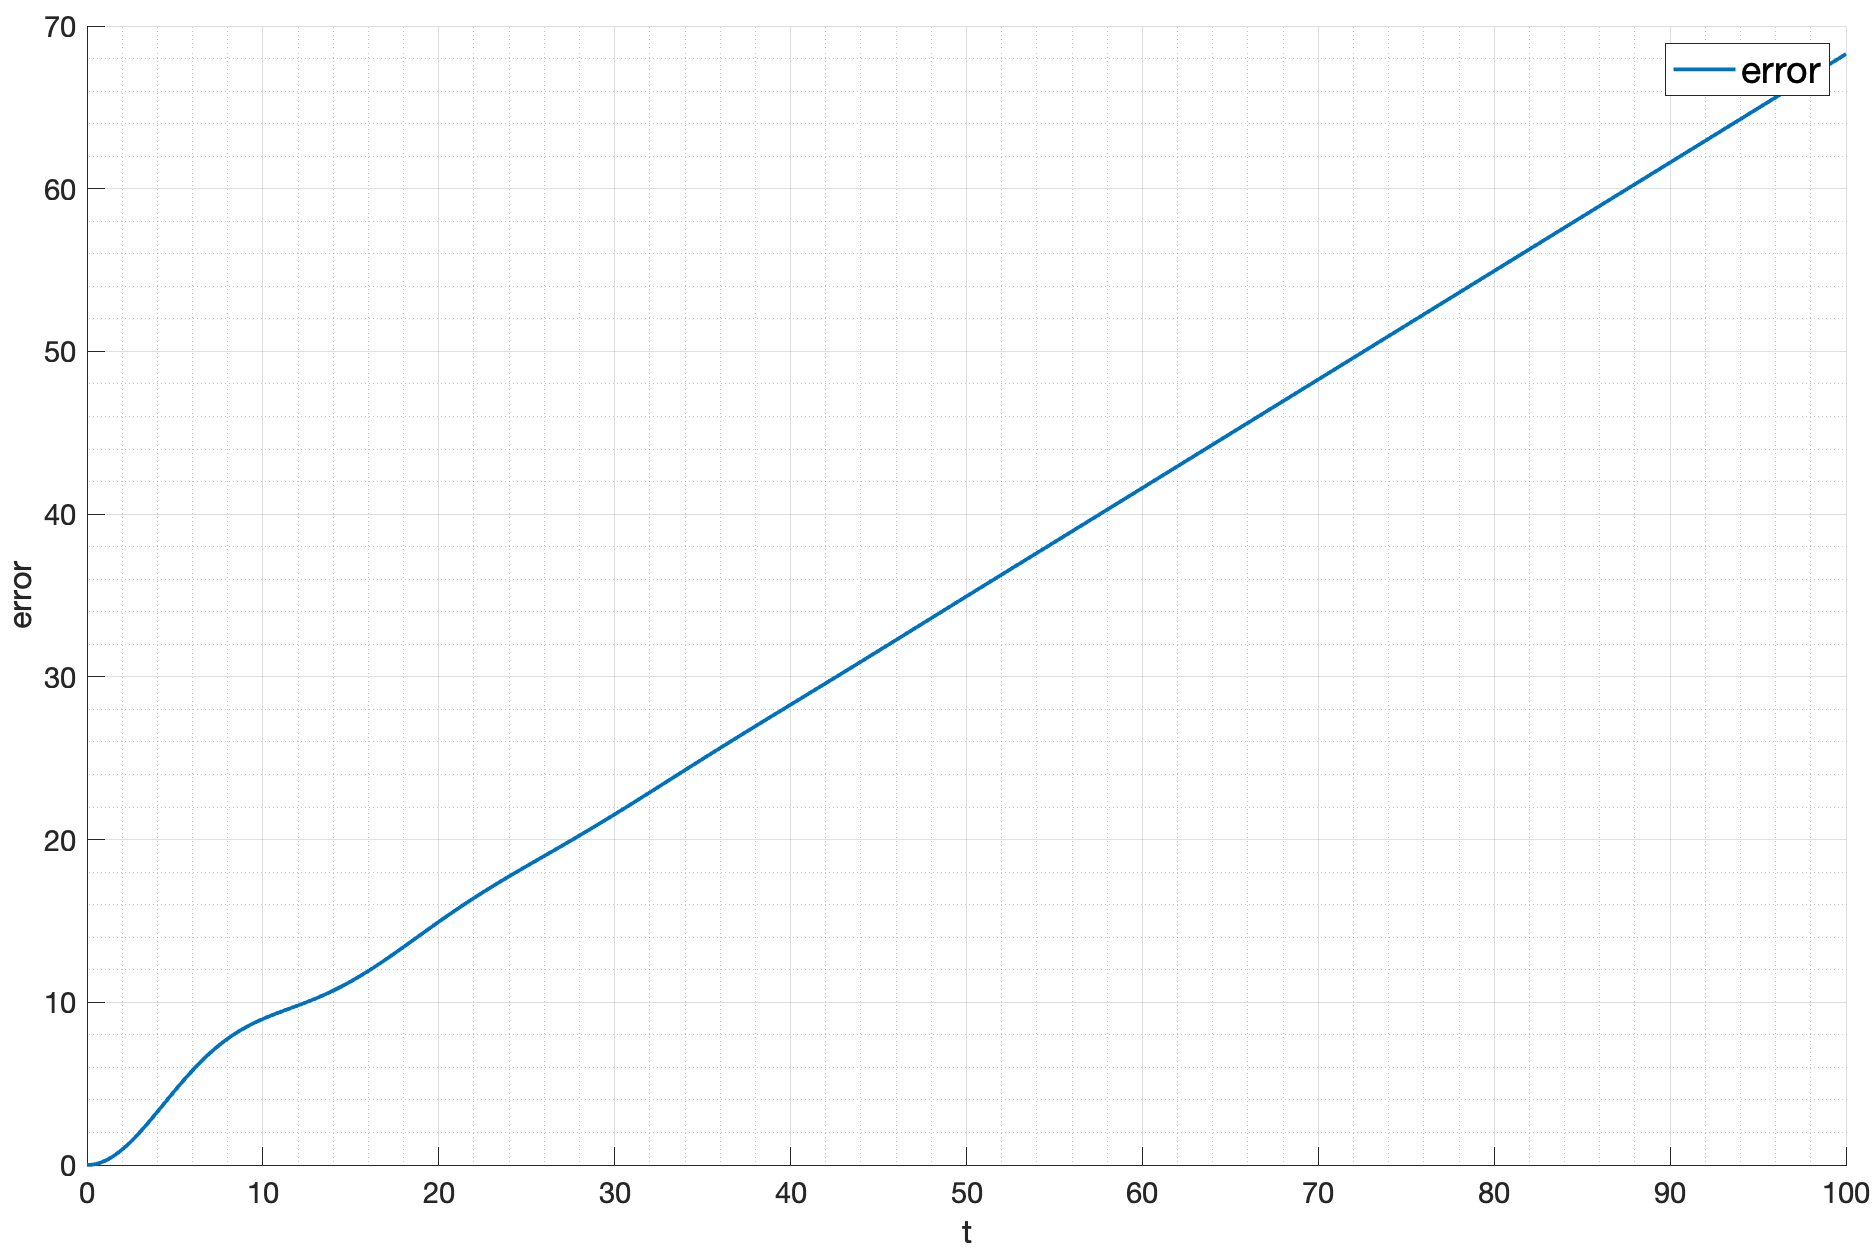
\includegraphics[width=\textwidth]{"media/plots/task4_error9.png"}
%     \caption{График ошибки системы с I регулятором ($k = 0.5$) ($u(t) = \frac{at^2}{2}$)}
%     \label{fig:task4_error9}
% \end{figure}

Видно, что во во всех случая ошибка нарастает, что подтверждает то, что система является астатической первого порядка. 

\FloatBarrier
\subsection{Вывод}
В данном пункте была рассмотрена система с I регулятором, который позволяет получить систему с астатизмом первого порядка.
Было найдено теоретическое значение установившегося значения ошибки, которое совпало с фактическим значением.
Для квадратичного выходного воздействия было показано, что ошибка не сходится к значению, что подтверждает астатизм первого порядка.